\chapter{Euch zum Geleit}

\chapter{Auf ein letztes Mal}

Lieber Waldemar,

Dieser letzte Teil der Geschichte wird wohl am kürzesten und fragmentiertesten ausfallen. Von den Ereignissen auf der Queste nach den Sieben Kelchen, der Begegnung mit den Trollen, und der grausamen letzten Schlacht sind kaum noch Berichte zu finden.
Dennoch konnte Aria mir zumindest einen extrem detaillierten Bericht über die Schlacht auf den Vallusanischen Weiden schicken, den Temyr verfasst hatte.
Auch wenn es vielleicht ein Vorurteil ist, aber ich denke, er beweist einmal wieder das Tulamiden unter all den vielen Völkern auf Deren die Wordgewandtesten sind.

Bitte füge die nächsten Zeilen nicht deinen eigenen Berichten zu, sondern verbrenne sie nachdem du diesen Brief erhalten hast. Ich muss dir von einer Geschichte erzählen, die vor einigen Wochen geschehen ist, aber niemand darf von ihr erfahren.

Seit Jahren hatte ich wenig von Temyrs Witwe Aria gehört. Die letzte Information, die ich hatte, war dass sie nach Khunchom gezogen war. Nach der Schlacht hatte sie wohl mehrere Jahre in Draknoia verbracht und bei den Elementarmeistern studiert. Aber nach diesem Exil hat sie eine Stelle an der Akademie in Khunchom angenommen, und ist wohl eine enge Vertraute der Akademieleiterin.

Ich hatte nur wenig Kontakt zu ihr, und sie war immer recht kalt in ihren Briefen. Ich hatte vermutet, dass ihr Schmerz um den Tod ihres Ehemannes einen Kontak zu mir, oder zu anderen Gefährten aus der Zeit Klammsbrücks zu schmerzhaft für sie machte, und hielt es daher für höflich, nicht aufdringlich zu werden.
Aber mein Projekt, und das der Rhodensteiner, drang immer mehr in jene Zeit vor in der auch sie Teil der Geschichte wurde, und so beschloss ich im Zuge einer Studienreise einen Abstecher nach Khunchom zu machen. Ich wollte die Gelegenheit ergreifen in Temyrs Geburtsort ein paar Nachforschungen anzustellen. Im Zuge dessen erschien es mir angemessen, ihren Wohnort zu erfragen und sie um ein Gespräch zu bitten.

Doch dazu sollte es zuerst nicht kommen! Es war ein heißer Herbstabend, und ich hatte den gesammten Tag in der Akademie über Berichte über den Dämonenkrieg gebrühtet. Mein Tulamyd ist über die Jahre leider sehr rostig geworden, ohne Temyrs blumiges Fluchen in unseren Hallen, und so zog sich meine Arbeit bis zur späten Stunde hin. In der Art alter Menschen vergaß ich, dass es eigentlich zu spät für einen freundlichen Besuch war, und machte mich auf zu Arias Stadthaus.

Als ich auf die Tür zuging, fiel mein Blick durch ein Fenster. Ich weiß, es ist nicht die feine Horasische Art, aber die Neugierde war immer meine größte Sünde. Normalerweise würde ich einer alten Freundin auch nicht nach spionieren, aber was mich erblickte erstaunte mich so, dass ich nicht anders konnte als vorsichtig zu lauschen. Bitte verzeih mir dies!

In Arias Empfangszimmer saßen mehrere in lange, graue Reisemäntel gehüllte Gestalten. Elementarwesen servierten dampfende Getränke, doch das war nicht das auffälligste. Einer von ihnen saß so, dass ich sein Gesicht halb erblicken konnte, und das war es, was mich wie Rondras Donner traf: elfische Züge, die blasse Haut eines Nordmanns, und eine Augenklappe. Es war Firnen! Ich weiß, es ist unmöglich, aber ich schwöre dir, es war Meister Wulfgrimm. Seine Haut war dünn, fast schon Pergamentartig, und seine gesammte Gestalt hatte einen etherischen Character an sich, ich kann es nicht besser beschreiben.

Ich konnte nicht viel vernehmen, aber sie sprachen von Splittern und den Heptarchen! Mir wurde schnell bewusst dass ich nichts davon hören sollte, und ich schlich mich feige davon.

Als ich am nächsten Tag, zu angemessener Stunde, Arias Haus erneut aufsuchte, wurde ich freundlich, aber immernoch etwas kalt empfangen. Aria spielte eine perfekte Gastgeberin, lenkte aber von allen Fragen nach Firnen und Temyr geschickt ab. Ich denke auch um mich ruhig zu stellen gab sie mir den Bericht ihres Ehemannes von den Vallusanischen Weiden und schob mich mit diesem in den Händen fast schon zur Tür hinaus.

Ich werde weitere Nachforschungen antreten und dir als bald von ihnen berichten. Bis dahin überlasse ich dir das Ende meiner Arbeit hier, den finalen Abschnitt über das Wirken der Gezeichneten.

Dein alteer Lehrmeister,\\
Iliricon Tannhaus


\chapter{Die Schlacht auf den Vallusanischen Weiden}

\section{Geleitwort}

\begin{flushright}
Claas Völcker, Toronto, den 
\end{flushright}

\section{Die Tagebücher}

\subsection{Aufzeichnungen des Temyr ibn Sahid}

\paragraph{24. Praios im Jahre 1020 nach Bosparans Fall}
Das Schicksal, werte Freunde, mag launisch sein, aufbrausend und zürnend, gewiss; aber es ist auch ein sturer, unbeirrbarer Herr. Und wiewohl man es auch zu täuschen gedenkt, man täte besser daran, einen tulamidischen Basarhändler auch nur um einen Schekel des gebotenen Preises beschwatzen zu wollen. Denn sobald es sich über seinen eigensinnigen Weg bewusst wird, weicht es keinen Zoll davon ab, und treibt das Weltgeschehen munter vor sich her. Was hierzu gesagt werden soll und muss: Unter den Männern und Frauen im Lager hatte man es leider versäumt, diese Weisheit zu verbreiten. Schon seit unserer überraschenden Einkunft hatten sich die Anzeichen auf die bevorstehende Schlacht gehäuft, bevorzugt in Form von Aaskrähen und anderer Galgenvögel, die sich auf den Ästen der entfernten Baumruinen lautstark um die besten Plätze für das anstehende Blutmahl rissen. Und ebenso eifrig hatte man versucht, die Boten und ihre Botschaft zu ignorieren. Wohin einen die nervösen und vor Erschöpfung zitternden Beine auch trugen -- denn zu schlafen vermochten nur die Toten -- überall versicherte man sich wort- und umfangreich der eigenen Seelenruhe. An den blakenden Feuern versammelten sich alle naselang Kämpen, Feldscher oder einfache Bader und ergingen sich im Kartenspiel. So einer einen Stich gesetzt hatte, was nur selten geschah, da niemand einen Blick auf den Verlauf des Spiels verschwendete, klaubte er mit dramatischen Gesten die Karten zusammen und bemerkte mit schriller Stimme, welches Glück ihm Phex da doch wieder an die Hand gegeben hätte. Nein -- von der Hoffnung, die vor zwei Tagen gleichsam mit unserer Ankunft in das Lager geweht ward, ist nicht mehr viel verblieben, und der klägliche Rest passt mühelos in einen namenlosen Holzsarg. Verzeiht meinen hässlichen Ton, tapfere Freunde, doch ich mag mich kaum der erschreckenden Eindrücke erwehren, derer ich alltäglich Zeuge werde. Es liegt der Duft der Verdammnis in der schwülen Hitze, welche unbarmherzig auf dem Heerlager liegt, wiewohl doch eisige Kälte ums Herz herrscht. Mehr noch, ein sehr bestimmtes Gefühl hat sich auf meine Seele gelegt, und das war noch nie ein gutes Zeichen. Ob es die astralen Präsenzen sind, die vom Feind herüberwehen und in meinen Ohren schreien, oder die Flut dunkler Wolken, welche das Firmament benetzen, weiß ich nicht -- wohl aber, dass es mich mit rasender Angst erfüllt. Der morgige Tag wird zeigen müssen, ob das Zeitalter der Menschen wirklich Bestand hat, oder aber unweigerlich der Verderbnis geweiht ist\dots

\paragraph{25. Praios im Jahre 1020 nach Bosparans Fall}
Noch in der nämlichen Nacht schwärmten die Scharführer aus, und in aller Stille wurde das gesamte Heer auf der Vallusanischen Weide massiert: Wohl an die 3000 Männer und Frauen aus den verschiedensten Provinzen, Baronien und Markgrafschaften der Garethischen Krone; als da wären Berittene und Fußvolk der Schildlande Tobrien und Weiden, insonderheit Pikeniere und schwere Kavallerie; Ritterschaft aus den Stammlanden des Mittelreiches, dort Bogenschützen im Verein mit Kürassieren, Plänklern und weiteren Gerüsteten; und die natürliche Vielzahl an gemeiner Infanterie, leichte wie schwere, deren Erscheinung von regionalen und kulturellen Grenzen verschont bleibt. Unter den matten Augen der Gestirne wurden Zelte abgebrochen, Pferde gezäumt und Kutschen und Wagen bereitet. Schwertgurte wurden geschnürt, Platten und Brünnen sicher angepasst, Freunde nahmen ein letztes Mal Abschied. Feldscher und Wundärzte, Zeugwarte, Schmiede und Bader fassten ihre Instrumente mit prüfendem Blick und bereiteten sich auf die kommenden Stunden vor. Die Offiziere, die alldieweil durch Straßen und Gässchen der Zeltfluchten schritten, brauchten ihre Stimmen nicht sehr zu heben -- eine Totenstille lag in der Luft, die trotz der kriegerischen Aufwendungen kaum gestört wurde. Auch in unsere Schlafstatt schlüpfte zu gegebener Zeit ein Knabe -- er mag kaum mehr als 14 Götterläufe gezählt haben -- und hieß uns aufstehen. Die Gewissheit der baldigen Schlacht wrang meinen Magen wie ein allzu nasses Tuch, so dass ich keinen Bissen der kargen Ration hinunterbekam. Meine Gefährten hatten dessentwegen aber durchaus keinen Vorteil, denn das Frühstück zählte ohnehin nur einen Bissen. Der erdrückenden Dunkelheit überdrüssig hätte ich wohl gerne ein Feuerchen entzündet, doch ebendies war allen Kämpfern strengstens untersagt worden.

``Ein Feuerschein, zumal in dieser Gegend,'' hatte Ayla am Tage unserer Ankunft vor ihren Generälen doziert, ``kann meilenweit gesehen werden und dem Feind wichtige Hinweise auf unsere Truppenbewegungen und Aufstellung geben. Auch wenn euch nach Licht dürstet -- vor der Offensive will ich Feuersteine und Stahl sicher in Taschen und diese Taschen fest verschlossen wissen. Verstanden?''
Und ein jeder hatte sich nun eilig bemüht, ihrer Aufforderung nachzukommen.

Über die flache Graslandschaft der Auen ließ sich der Blick tatsächlich mächtig weit schweifen, so dass man nicht umhin kam zu bemerken, dass auch das gegnerische Lager in hektische Betriebsamkeit ausgebrochen war. Die tausendfachen Schemen verschwommen im nebligen Halbdunkel zu einer einzigen, vielarmigen Gestalt, die ihre widerlichen Auswüchse gierig nach uns streckte. Nicht nur ob der nächtlichen Kälte zitternd bezogen wir schließlich die uns zugewiesene Aufstellung bei der Heerführung. Während die Tausendschaften an Soldaten aus allen Winkeln des Lagers zusammengezogen wurden und schweigend Aufstellung bezogen hatte ich ausreichend Muße, mir die Dimensionen und geographischen Feinheiten des Kampfplatzes in Erinnerung zu rufen. Denn wiewohl ich freilich kaum etwas davon zu erkennen vermochte, so hatte ich doch den letzten Tag genutzt, mir die Landschaft einzuprägen.

Zu unseren Füßen erstreckten sich die nördlichen Ausläufer der Vallusanischen Weiden hinab in eine flache Talsohle, welche weit im Süden vom Wasser eines mächtigen Stromes zerschnitten wurde: der Misa. Schnurgerade wie ein Schwerthieb teilte der Fluss die beidseitigen Steppen, die bis an seine Ufer mit dichten Farnbüschen und Gräsern bewachsen waren und in glücklicheren Zeiten allerlei Viehzeug zum Äsen gereicht hatten. Gen Osten setzte sich diese Flora beharrlich fort, bis die dichte Grasdecke schließlich unversehens abriss und Morasten und Schilfpflanzen wich; die Misa selbst jedoch mündete dort in die Tobrische See. Hier, ein Dutzend Meilen stromaufwärts, saß die Stadt Vallusa, deren Außenmauer keck an das Südufer des Flusses drängte. Darin eingefasst, von Türmen und Lagerschauern bekränzt, präsentierte sich der Hafen, gleichsam Lebensader wie Stolz Vallusas. Als letzter Umschlagplatz für auf der Misa geschiffte oder geflößte Waren vor dem Meer hatte die Stadt schon früh ihre tragende Rolle im Nah- und Fernhandel wahrgenommen; auch konnte man sich hier mühelos nach Medina oder gar Perricum einschiffen, und alsbald erfreuten sich die Ratsherren ihrer Einkommen aus der zivilen Seefahrt. Nun jedoch lagen die sonst so betriebsamen Docks und Stege, die Kontore, Kaimauern und Werftplätze in aller Stille da. Die Hafenpforte war verschlossen und mit Schutt und Geröll verstopft worden, während auf den Wehrgängen und in den Wachstuben eifrige Betriebsamkeit herrschte -- so zumindest tat es der Fackelschein kund, der allgegenwärtig auf der Stadtmauer kreiste. Die Armee der Notmärker hatte ihre stählernen Finger um die Stadt geschlossen und drohte nun, diese allmählich und qualvoll zu ersticken. Bislang hatte man noch keine Anstrengungen unternommen, die Mauern im Sturm zu nehmen, doch die Kollaborateure hatten sorgsam alle Versorgunglinien entlang der Misa abgeschnitten, wodurch die gesamte Lebensmittelversorgung auf einmal verlustig ging. Gleichzeitig liefen unsere eigenen Truppen, die gemäß des Schlachtplans frühzeitig auf die südliche Seite des Flusses übersetzen sollten, somit beträchtlich Gefahr, einer weiteren Übermacht ausgeruhter Söldlinge in die Arme zu laufen.

Rückwärtig, bereit zum Schlag, befanden sich die beiden Heerlager des Helme Hafax, derer wir schon auf unserem abenteuerlichen Ritt durch die Lüfte ansichtig geworden waren. Das nördlichere von beiden lag verborgen hinter einer aufragenden Hügelkette, noch geschützt von einem Ausläufer Waldes, das andere hingegen bedrohte von Osten her unsere Flanke.

Endlich hatten sich unsere Kämpfer postiert und ihre vorläufige Aufstellung eingenommen. Über ihren Köpfen flatterte eine Vielzahl von Standarten und Bannern, Wimpeln, Fahnen und Flaggen von unterschiedlichster Herkunft im sanften Wind. Die Pferde scharrten aufgeregt, nervöse Blicke blitzten unter den Visieren und Helmen hervor. Eine Woge der Unruhe strich über die versammelten Männer und Frauen, und nicht wenige erhoben ihre Stimme zu einem angstvollen Flüstern. Firnen, der diese Verzweiflung wohl spürte, trat entschlossen vor, und in die plötzliche Stille hinein erklang seine Rede, die tausendfach in den Herzen und Köpfen der Truppen wiederhallen sollte:

``Tapfere Männer und Frauen Aventuriens, Brüder, Schwestern, Gefährten\dots Schreckliches ist euch in den letzten Monden wiederfahren. Viele von euch haben verloren, was ihnen lieb und teuer war, Kameraden, Freunde, die Heimat\dots Ihr alle habt in diesen grausamen Abgrund gestarrt, an dem wir uns heute befinden, ihr alle habt die hässliche Fratze des Krieges gesehen, die höhnisch auf euer Opfer herabschaut. Und es mag Zeiten gegeben haben, in denen ihr gezweifelt, verzagt habt. Ihr weder Mut noch Zuversicht verspürt habt, sondern nur noch grenzenlose Angst. Ihr alle kennt dieses Gefühl der Machtlosigkeit\dots Und doch steht ihr heute versammelt, das Schwert in der Rechten und das Siegel des Bundes über dem Herzen. Wir alle müssen uns unseren Dämonen stellen. Nicht die Klingen und Speere der Feinde sind es, die uns etwas anhaben können. Nicht ihre frevlerischen Rituale vermögen es, unseren Willen zu erschüttern. Nein, es ist die Furcht, die wir im Herzen tragen, welche die schlimmsten Wunden reißt. Wir selbst sind es, in denen der Samen des Zweifels keimt. Und doch steht ihr heute versammelt\dots Ihr alle habt die schlimmste und grausamste Schlacht bereits geschlagen. Ihr habt über euch selbst triumphiert. Diese Zuversicht, diese Rüstung der Hoffnung ist es, die uns wirklich leben lässt. Und deswegen ist es gleich, wie viele sich uns heute in den Weg stellen werden, es ist gleich, wie oft sie uns niederstrecken werden. Denn was auch geschieht, wir werden aufstehen und kämpfen. Unsere Knochen mögen zerbrechen und unsere Arme schwer vom Kampf werden, aber niemals werden sie die Hoffnung in unseren Herzen töten.''

``Brüder und Schwestern, heute ist der Tag gekommen, an denen wir es diesen Bastarden hundert- und tausendfach zurückzahlen werden. Ihr seid die Klinge der Hoffnung Aventuriens, ihr seid die Heimat der Heimatlosen, ihr seid das Licht in finsterer Nacht. Vor den Augen von Menschen und Göttern werden wir heute Geschichte schreiben. Selbst wenn wir sterben, die Welt wird diese Schlacht nie vergessen. Niemand wird euch je vergessen. Für unsere Familien, für unser Land, für die Zwölfe!''

Niemand regte sich nach dieser Ansprache, kein zustimmendes Gebrüll zerriss die Stille des frühen Morgens. Doch in den Augen der Männer und Frauen glomm Entschlossenheit, und wie zur Antwort wurden Lanzen und Schwertschäfte mit nunmehr festem Griff gepackt.

``Wohl gesprochen, Meister Wulffgrimm'', bemerkte Ayla, als sie ebenfalls vor die Reihen der Kämpfer trat. Ihr goldenes Haar tanzte im Wind und umspielte die brüllenden Löwen, die ehern auf ihrem Brustpanzer ruhten. Selbst im matten Schein des Madamals glänzten die goldgewirkten Ziselierungen, die kunstvoll den schützenden Stahl überzogen und die würdevolle Leuin auf dem Wappenrock umrahmten. Am Gürtel hing der viel besungene Löwenhelm, dessen Nackenschutz als üppige Mähne über die Flanken des Schwerts der Schwerter fiel. Ein wahrhaftiger Löwe hätte nicht stolzer den Boten der Göttin ausfüllen können, als Ayla vom Schattengrund ihre Stimme erhob und begann zu singen. Und wie ihr Lied sanft den Morgennebel durchflocht, da brannte ein Feuer in meinem Herzen auf, so stark und gleißend, dass ich hätte vergehen müssen. Aber die Flamme verschlang nicht, versehrte nicht, vielmehr erfüllte sie den ganzen Körper mit lebendiger Wärme. Denn es war die Flamme der Zuversicht, die Ayla mit ihrer Liturgie entfacht hatte, und kein Schrecken der Welt hätte die Mauern dieses Tempels einreißen können. Dunst und Nebel zerrissen, als hätte man sie mit dem Schwert zerteilt, und immer noch sang Ayla ihr einsames Lied, ließ die Melodie über die Köpfe des Heers wehen. Ich schloss die Augen und lauschte, gab mich dem Klang ihrer Stimme hin. Mein Körper wurde von immer neuen Wogen der Empfindung umspült, die unerbittlich an den Felsen der Zweifel und Angst rissen und diese mühelos hinfort trugen, weit, weit fort, in ein fernes, früheres Leben. Warm erschall Aylas Stimme in meinem Innern. Kein Zweifel, keine Angst, kein Bedauern. Wahrlich, keine irdische Stimme konnte so singen. Der Faden der Melodie wurde dünner und zitternder, mein träumender Geist fiel hinab in seine diesseitige Hülle, und ich öffnete die Augen. Kaum hörbar verlor sich das Lied in der Morgenluft. Da riss das Schwert der Schwerter die legendäre Klinge Armalion aus der Scheide, und reckte den Zweihänder gen Alveran. Und wie zur Antwort wurden tausende Schwerter und Lanzen gleichsam erhoben, und goldene Sonnenstrahlen überfluten den gezückten Stahl, wiederspiegelten auf Rüstung und Schilden. Der Tag der Entscheidung war endlich angebrochen.

Der dumpfe Hall von Trommelschlägen begleitete die weitere Anordnung und Aufstellung der Kämpen und kündete unmissverständlich vom Aufzug des Feindes. Während die Fußkämpfer bei ihren Offizieren Stellung bezogen und lautstark in der Schlachtenordnung unterwiesen wurden, führte uns der Weidener Bär zu einer Kompanie, die etwas abseits ihres Einsatzes harrte.

``Dies sind die berühmten Drachenpforter Schützen!'', verkündete Waldemar ohne Umschweife und wies mit der Hand auf die bunt zusammengewürfelte Truppe, die sich da vor uns präsentierte. Sie trugen Panzer aus dunklem, steifem Leder, die auf Brust und Rücken mit zusätzlichen Nieten verstärkt waren. Darüber hing ein Gewirr aus Gürteln, Schlaufen und Feldtäschchen, welche die Schützen mit allerlei nützlichen Gerätschaften, insbesondere Bolzen, bestückt hatten. Die zugehörigen Armbrüste steckten in eigens gearteten Gehängen an Hüfte und Rücken, manch einer führte gleich mehrere davon mit sich. Den Tag zuvor hatte Waldemar so manches Wort über diese Waffen verloren, und sich dabei in umfänglichen Erläuterungen der verwendeten Hölzer und Spannmechanismen ergangen; er war auch nicht müde geworden, den Eifer und die Zielsicherheit zu benennen, welche ``seine Jungens'' seinem Wort nach im Umgang mit den Schusswaffen an den Tag legten: Diese hier verfügten am Steg über Umlaufrollen, an deren innseitiger Achse eine Kurbelwelle angeschweißt war. Die Sehne aus Tierdarm wiederum umspannte einen gelagerten Schlitten, dessen rückwärtig eingefasste Rippenstange über die Achsenwelle hinweg lief. Drehte man nun an den beiden Kurbeln, so wurde die Sehne allmählich eingeholt und schließlich am Ende des Handlaufs arretiert. Aber ich will euch nicht weiter mit mechanischen Feinheiten langweilen, werte Freunde!

Weiterhin boten die Hüftgurte Platz für eine Vielzahl von Kurzschwertern, Dolchen, Stiletten, Jagdmessern und weiteren Sehnenschneidern, welche die Unterschiedlichkeit ihrer Träger noch einmal lebhaft unterstrich: Die Truppe zählte wohl an die 20 Männer und Frauen, die scheinbar aus allen möglichen Enden Aventuriens in diese eigenartige Mannschaft geraten waren. Es war, als hätte man bei der Gründung der Truppe die Vielseitigkeit zur Prämisse erhoben und aus dem kulturellen Eintopf der Mittelreichischen Gesellschaft jeweils einen Vertreter geschöpft. Zwerge tummelten sich da neben Elfen, Halblingen und Menschen, raue Nordlichter überprüften gemeinsam mit feingliedrigeren Garetiern ihre Ausrüstung. Die Drachenpforter Schützen indes sollten schon bald Gelegenheit haben, uns ihrer Einheit im Felde zu versichern.

Angeführt wurde dieser lustige Haufen von einem drahtigen jungen Mann mit Pagenschnitt und Vollbart, welcher Rondrigan Wolf geheißen wurde und bis auf gelegentliches Blecken der Zähne kaum eine schlechte Angewohnheit von seinen tierischen Vettern übernommen hatte. Hauptmann Wolf erwies sich rasch als wesentlich bedächtiger und zurückhaltender, als es die Schilderungen seines Lehnsherren vermuten ließen; gleichsam war er sich jedoch nicht zu schade, in die Begeisterung bezüglich seiner Truppe einzustimmen.

``Wir sind auf schnelle Vorstöße spezialisiert'', erläuterte er uns fachmännisch, als Waldemar endlich gegangen war. ``Kundschaften und Nadelstiche setzen -- das ist unser Terrain auf der taktischen Karte. Für wohlfeile Strategien ermangeln wir uns an Mannstärke, und der Zweikampf ist unsere Sache nicht, zweifellos. Aber unsere Schlagkraft liegt in der Beweglichkeit, in der präzisen und unverzüglichen Erstickung von Gefahren. Wir meiden das Armdrücken, und schießen den ganzen Arm lieber aus hundert Schritt mit einem Bolzen entzwei.'', setzte er lakonisch hinzu und tätschelte seine eigene Armbrust. ``Kein Wunder, dass uns die Leuen nicht sonderlich mögen\dots'' Und mit einem vielsagenden Blick wies er auf die Kompanie an Rondra-Geweihten, die in der Ferne Stellung bezogen.

Alsbald die Drachenpforter Schützen unter den Befehlen ihres Hauptmanns Waffen und Ausrüstung bereitet hatten, wurden die Gürtel fester geschnürt und der Aufmarsch begann. Im hohen Gras verborgen näherte sich unsere Kompanie rasch, aber stets umsichtig der nördlichen Hügelkette, welche sowohl das zweite Lager als auch die Absichten des Feindes dahinter trefflich verbarg. Allenthalben wehte der Wind Fetzen der Schlacht heran, die im Schoße des Weidlandes angebrochen war. Schwerter klirrten, Hörner gellten, Schmerzensschreie zerschnitten die kühle Morgenluft. Es war die perverse Symphonie des Todes, orchestriert auf Lanzen und Bogensehnen, geschrieben mit dem Blut Gefallener. Ein weiteres Mal beschlich mich jenes ungute Gefühl, dass sich seit dem Vorabend wie selbstverständlich in meinem Herzen einquartiert hatte. Schon färbte sich die Erde unter den Soldatenstiefeln dunkel von Blut, wiewohl des Hauens und Stechens noch keine der beiden Seiten ermüdete. An vorderster Front jagte Ayla mit ihren Getreuen umher und hielt unter den Borbaradianern reichliche Ernte; eine Woge aus Rot und Gold, die einer Flammenzunge gleich unter den Feinden wütete und allzu kühne Vorstöße verbrannte. Doch es zeigte sich rasch, dass die zahlenmäßige Überlegenheit unseres Gegners nicht so leicht aufzuwiegen war. Um die Geweihten herum fielen die Söldlinge wie Fliegen, gewiss, aber die klügeren unter ihnen umschwärmten den tödlichen Stachel einfach und breiteten sich über eine viel weitere Kampfeslinie aus. Dadurch entgingen sie nicht nur den todbringenden Schwertern der kampferprobten Rondrianer, sie brachten auch den Rest unserer Truppen in arge Bedrängnis. Auch uns erwartete ein nämliches Schicksal, denn Schwadronen berittener Kämpfer, denen der Durchbruch an der Frontlinie geglückt war, kreuzten im Rücken des Heeres und suchten nun, versprengte Einheiten aufzureiben. Der Deckung so plötzlich beraubt erschien unser Tross gar zu auffällig; und nur mit wahrhaft phexischem Glück gelang es uns, bis zu den Säumen der Hügel den Schergen zu entgehen.

Wir hatten jedoch nicht viel Zeit, der gütigen Vorhersehung unseren Dank auszusprechen, denn von den Gipfeln der Erhebung dräuten bereits die feindlichen Onager. Es waren jener drei; mächtige hölzerne Maschinen, die wie Gerippe aus der Grasdecke empor stachen. Sie waren noch im Aufbau begriffen, wie die emsige Betriebsamkeit zu ihren Füßen nahelegte, doch es war nur eine Frage der Zeit, bis ihre Geschosse unsere Reihen zerpflücken würden. Zum Installationstrupp hinzu gesellte sich eine Vielzahl weiterer Gestalten, deren Kleidung und Bewaffnung sie unzweifelhaft als Angehörige der mechanischen Zunft ausschloss.

``Wartet'', ließ sich Hauptmann Wolf vernehmen. Er zog aus den Untiefen seiner Gewandung eine lederne Tasche, in welcher sich eine Handvoll Kugeln befand. Die Kugeln selbst waren aus Ton gefertigt und mit einer geteerten Zündschnur versehen, die ihren Verwendungszweck allzu offenkundig unterstrich. Natürlich hat jeder von euch, werte Freunde, schon einmal von den Hylailer Feuerkugeln gehört; ich selbst kenne ein Dutzend Alchemisten, die sich beim Versuch ihrer Herstellung in die Luft gesprengt haben.

``Ihr mögt mir glauben, dass meine Schützen im Werfen ebenso geschickt sind wie im Umgang mit der Armbrust. Doch zuerst müssen wir die Wachmannschaft ausschalten.'' Schnell und bündig wurden die entsprechenden Befehle verteilt, und nur einen Augenblick später hatten die Drachenpforter Schützen ihre Feldformation eingenommen: Zwei gegeneinander verschobene Linien, sodass seitlich hinter den Vordermännern jeweils versetzt ein weiterer Kämpfer stand. Davor freilich präsentierte sich Rezzanjin, den auch die engelszüngigen Reden und Argumente Hauptmann Wolfs, er werde sich noch ``ein weiteres Arschloch'' einholen, nicht von seinem angestammten Platz vertreiben konnten. Der Rest unserer Kompanie ordnete sich der Empfehlung des Hauptmanns gemäß sowohl im Rücken als auch an den Flanken der Aufstellung ein, um Übergriffe nach allen Seiten hin abschirmen und selbst ``ordentlich austeilen'' zu können. Dann begann der Sturm auf die Hügelspitze. Die feindlichen Plänkler indes begrüßten diesen Vorstoß mit wildem Geschrei und schickten sich an, uns mit Schwert und Schild gebührend zu empfangen. Sie hatten die Rechnung allerdings ohne Rezzanjin gemacht, welcher in Windeseile den Anstieg genommen hatte und nun wie ein Derwisch unter den verdutzten Söldlingen wütete. Die aufgescheuchten Männer wichen hastig vor der wild fahrenden Klinge zurück, die Kettenpanzer, Fleisch und Knochen mit grausamer Leichtigkeit zerriss und nur als schwarzer Schemen leidlich zu erkennen war, so schnell wurden die Hiebe geführt. Die angststarren Krieger wiederum boten vortreffliche Ziele für die Bolzen der Drachenpforter Schützen, und manch einer verschied, ohne auch nur einen Streich mit dem Schwert geführt zu haben. Warmes Blut lief den Abhang entlang. Doch eine Überzahl von Dreißig erfahrenen Recken ist auch in der Überraschung nicht so leicht aufzureiben, und die Borbaradianer hatten, trotz des Schreckes, ihr blutiges Handwerk nicht verlernt, wie sie in dem nachfolgenden Hauen und Stechen eindrucksvoll unter Beweis stellten. 

Rezzanjin wurde von vier Mann gleichzeitig in die Zange genommen, während zwei weitere unentwegt auf Irians Schild einhämmerten. Aufstellung und Ordnung waren längst verlustig gegangen, und die Drachenpforter erwehrten sich mit Messern und Säbeln der feindlichen Klingen. Hauptmann Wolf indes versicherte sich von der Nahkampftauglichkeit seiner Armbrust, vermittels welcher er seinem Gegner den Schädel einschlug. Auch das Aufbaukommando hatte sich inzwischen zu den Kämpfen gesellt. Es waren, wie ich mit Schrecken feststellte, nicht Menschen, sondern fahle Gerippe, mit Resten verdorbenen Fleisches behangen. Ein irres Licht brannte in den blutverkrusteten Schädeln und lies den Umstehenden von niederhöllischer Kälte das Herz gefrieren. Ich warf Firnen einen raschen Blick zu: Wir beide wussten nur allzu gut, dass die Erweckung und Kontrolle von Leichnamen immer die Anwesenheit eines Magiers erforderte, eines Puppenspielers, der seine Marionetten zum wahnsinnigen Tanz führte. Wie zur Antwort erscholl ein gellender Schrei: ``Fulminictus!'', und einer der Drachenpforter Schützen stürzte, von einem unsichtbaren Pfeil niedergestreckt, zu Boden. Bis zur Kappe des Hügelkamms waren es noch einige Schritt den Hang hinauf, doch irgendwo dahinter musste der Magus lauern. Wir nahmen den verbliebenen Rest des Anstiegs und sahen uns nicht einem, sondern drei Magi gegenüber, in dunkle Roben gehüllt, auf denen das rote Zeichen des Dämonenmeisters prangte. Einer hob die Hand und bereitete sich auf einen vernichtenden Cantus vor, doch Ragnos hatte die Lage blitzschnell erfasst und jagte ihm einen Pfeil zwischen die Augen. Noch bevor sein toter Leib die Erde berührte ließ Firnen ein flammendes Schwert auf den nächsten Unglücklichen herabfahren, welches ihm einen furchtbaren Hieb über die Brust versetzte und nicht viel mehr als zwei verbrannte Hälften übrig ließ. Der Dritte im Bunde wandte sich zur Flucht, stürzte den Hang hinab und wurde dort von den Drachenpforter Schützen, welche die verbliebenen Gegner zerlegt hatten, niedergemacht.

Schwer atmend und von Schweiß überströmt standen wir zwischen den Leichen der Borbaradianer und maßen unseren eigenen Blutzoll. Viele hatten Verletzungen davongetragen, doch wie durch ein Wunder war kein einziger in die Hallen des Todesgottes eingekehrt. Es blieb jedoch nicht recht Zeit, ob dieses erfreulichen Umstands die Glieder zu strecken, werte Freunde, denn schon nahte von Süden her ein weitaus größeres Übel: Zunächst kündigte es sich nur durch Donnern an; das schwere Donnern einer Vielzahl beschlagener Hufe. Dann sahen wir ihn, den waffenstarrenden Keil, der unerbittlich die Wiesen hinauf drängte und nichts zurückließ denn zerfurchte Erde. Ein Wald aus Lanzen spross aus dieser tobenden Masse heraus, ein wogendes Meer aus stählernen Speeren, manch einer mit blutigen Wimpeln und Bannern geschmückt. Dieser schnaubende Tross, vom Dröhnen und Klirren und Schreien angelockt, jagte in unerbittlichem Galopp über die Felder, und kein Dämonengezücht hätte einen fürchterlichen Anblick bieten können. Die erhitzten Rösser schnaubten vor Wut, und ihre Herren stimmten in den grausamen Choral munter ein. Der Beritt kam rasch näher, viel zu rasch, und allzu bald würde auf diesem Hügel ein zweites Gemetzel stattfinden\dots 

``Wie gut, dass auch wir noch ein paar Listen im Sack haben\dots'', meinte Firnen und brachte aus den Tiefen seines Gewands einen Ring hervor, welchen er sogleich über einen Finger gleiten ließ. Der Ring war von kaltem Weißgold und Mondsilber gefertigt, worin ein einziger Kristall Eises gefasst war. Es handelte sich um eines der Artefakte, welche Firnen und mir im Konzil der Elemente anempfohlen worden waren, und worin ein jedes einen Geist der Elemente barg. Firnen sprach sanft, wenngleich bestimmt: ``Zeige dich, Dschinn, Gebieter des Eises!'' Es wurde sofort merklich kühler, die Feuchtigkeit in der Luft legte sich in Schwaden über den Hügel, verfestigte sich in einem Wirbel aus Eisblumen und Schneefunken, der rasch menschliche Züge annahm. Klirrend entwuchs dem Ring die Gestalt, Arme sprossen aus dem scharf geschnittenen Leib wie Eiszapfen, und ein strenges Gesicht erhob sich über dem Körper, in dessen glänzenden Augen tausendfach das Sonnenlicht brach. Die Drachenpforter Schützen staunten mächtig, da sie dieses Wesens ansichtig wurden, doch Firnen wusste, was zu tun war. Er wies auf die Flanken des Hanges zu seinen Füßen, auf denen der morgendliche Tau schimmerte, und bat mit fester Stimme: ``Ich bitte dich, vereise sie.''

Ein eisiger Wind verwehte die Gestalt, zerstob sie in eine Woge schimmernder Kristalle, welche den Hügel hinunter floss und sich sanft auf die Gräser legte. Im Nu war die Wiese von einem zarten Umhang aus Silber bedeckt, einer spiegelglatten Fläche Eises, die sich bis ins Tal hinab zog. Johlend und kreischend brach die Kavalkade heran, begeistert stürzten die Pferde voran, und sahen unter ihren Scheuklappen nicht die Gefahr, die sich an den Boden schmiegte. Das vorderste Ross, dessen Reiter einen schwarzen Harnisch mit roten Intarsien trug, machte einen gewaltigen Satz und landete auf dem gefrorenen Gras. Die Hufe rutschten über das Eis, fanden zu ihrer Verwunderung keinen Halt und quittierten augenblicklich den Dienst, wodurch die ungestützten Fesseln ausbrachen und der Länge nach hinschlugen. Die nachfolgenden Reiter erkannten spät, viel zu spät die Gefahr und versuchten panisch, ihre Hengste auszubremsen, doch sie hatten die Fünfzig Mann hinter sich vergessen, die ungeduldig und mit Macht nach vorne drängten. So kam es, dass nicht nur die ersten unglücklichen Recken von ihrer eigenen Kameraden Pferde niedergetrampelt wurden, sondern sich die gesamte Reiterei in schönster Manier auf die Fresse legte. Dies vergönnte uns einen kurzen Moment der Ruhe, denn die Kavallerie hatte es durchaus nicht eilig, wieder auf die Beine zu kommen. Während die Männer unten fluchten und schrien hatten wir also ausreichend Gelegenheit, das weitere Vorgehen zu planen. Die Onager zu zerstören wäre nun ein Leichtes gewesen, doch hernach hätte uns der Beritt zweifelsohne auf die Hörner genommen, wie die zornigen Ausrufe lebhaft unterstrichen.

Mir kam eine Idee: Ich holte die Elementarringe hervor, die Firnen schon so trefflich eingesetzt hatte, und wählte einen massiven irdenen Ring aus, den man scheinbar direkt aus dem Granit des Raschtulswalls geschlagen hatte. Der Stein war warm und schien in meinen Händen zu pulsieren, als schlummerte eine große Kraft in ihm. Ohne zu zögern steckte ich mir das Artefakt an einen Finger und sprach das Losungswort: ``Erscheine!'' Sogleich ging ein Ruck durch den Hügel, ein dumpfes, tiefes Beben erschütterte den Kamm, Steine rollten den Hang hinab. Direkt vor mir brach die Erde auf, zerriss die flache Grasdecke und gab den Blick auf das felsige Herz des Berges frei. Daraus empor wuchs ein Mann, groß und dick wie ein Findling, auf dessen Brust sich Adern von Kupfer und Eisen streckten. Der Mund aber, werte Freunde, war angefüllt mit Diamanten und Schieferplatten, und als Augen glommen zwei Stück Eierkohlen. Er blickte auf mich herab und verschränkte die Arme vor seinem mächtigen Bauch. Ich blieb nicht lange reglos, denn ein Schrei des Hauptmanns gemahnte mich zur Eile. ``Dschinn des Erzes, Herr über Stein und Fels, ich bitte dich: Zerschmettere diese Onager und fege sie von deinem Hügel hinfort, stürze sie den Hang hinab und zerschlage unsere Feinde!'' Der Riese nickte bedächtig, dann schritt er zur Tat. Die gesamte Erhebung schien zu erzittern, als er mit mächtigen Schlägen die Onager einriss und ganze Brocken aus Holz und Stein die Flanken hinab warf. Die Berittenen, die rasend vor Wut und Hass ihre Pferde zurück gelassen hatten und zu Fuß den Anstieg wagten, blickten mit geweiteten Augen auf die Welle aus Geröll, Schutt und Steinen, die sich von der Hügelspitze unerbittlich ins Tal ergoss und über sie hereinfiel. Einige, die noch unten geblieben waren, gaben so schnell Fersengeld, dass die Tiere Mühe hatten, mit ihnen Schritt zu halten; wer sich jedoch nicht retten konnte, wurde von der Woge verschluckt und nicht mehr gesehen.

Nun waren zwar die Onager zerstört, doch der Rückweg gestaltete sich nicht minder schwierig. Die Drachenpforter hatten kaum ihre Reservearmbrüste gespannt, da stürzten unter furchtbarem Kreischen und Brüllen Rauchsäulen vom Himmel herab. Die brodelnden Schwaden zogen leckende Flammenzungen durch die Luft, die von schwelendem Sulphur und Ammonia rochen, und mitten in unsere Kompanie hinein fielen jene Gestalten, die man wohl Karakilim nennt. An die zwei Schritt hoch, in schwarze teerige Fetzen gehüllt, die Klauen bewehrt mit Schwertern und feurigen Peitschen. Ein unglaublicher Tumult brach aus, ein grotesker Tanz zwischen Menschen und Schatten, chaotisch beleuchtet vom Licht der gierig kreisenden Fuchsschwänze. Die Waffen der Dämonen schlugen schwärende Wunden, wie wir schon am eigenen Leib erfahren hatten, doch die Drachenpforter erwiesen enormes Geschick darin, den Finten und Hieben zu entgehen. Alsbald hatten sie auch ihren Schreck überwunden und landeten selbst großartige Treffer, so dass die niederhöllische Schar rasch aufgerieben war. Dort, wo die Karakilim an den Boden gepfählt oder von unzähligen Streichen erdolcht worden waren, brannte die Erde, Gräser verdorrten und faulige Pestilenz schlug pulsierende Ranken. Zügigen Schrittes ließen wir die Anhöhe hinter uns.

Es frischte merklich auf. Die anschwellenden Winde zogen in weiter Ferne mächtige schwarze Wolken zusammen und beugten jeden Grashalm demütig zu Boden. Wir hatten es gerade zur Hälfte des Feldherrenhügels gebracht, als es donnerte. Doch es war nicht das Gewitter, oh nein; vielmehr donnerte die Erde in altbekannter Manier, und mit stiebenden Hufen preschte die wieder formierte Kavallerie heran, im festen Willen, diesmal den entscheidenden Schlag zu setzen. Die Drachenpforter griffen erneut ihre Waffen, vor Erschöpfung schnaubend. Ich aber konzentrierte mich auf den Cantus Motoricus, spürte meine Arme wie von Blei ermüden, und schleuderte die Formel den nahenden Mordbuben entgegen. Der Ritt endete brutal, als hätten tausende unsichtbarer Hände die Reiter bei den Röcken gepackt. Wie ein riesiges Gewicht drückte das von mir heraufbeschworene Fesselfeld auf die Glieder der Borbaradianer, so dass jede ihrer Bewegungen der größten Anstrengung bedurfte. Derweil drängten die hinteren Reihen der Kavallerie, die rechtzeitig auszuweichen vermochten, um die magische Falle herum und setzten zum Angriff an. Doch Hauptmann Wolf und seine Leute hatten die Armbrüste bereits im Anschlag.

Wenige Minuten später war der Kampf beendet. Die Bolzenhagel der Drachenpforter hatten die Aufstellung der Reiterei gründlich zerlegt, und ehe ein einziger Borbaradianer unsere Linie erreichte, färbten schon zehn seiner Kameraden die Weiden dunkel mit ihrem Blut. Dieser aber traf uns umso härter. Und obwohl es uns schließlich gelang, die Plänkler mit Granaten und Schwertern zu zerreiben, musste doch ein Getreuer sein Leben lassen. Es sollte nicht der letzte bleiben.

Ohne weitere Scharmützel erreichten wir, reichlich erschöpft, den Feldherrenhügel. Vor den wachsamen Augen des Reichserzmarschalls Leomar vom Berg erstreckte sich hier das gesamte Schlachtfeld bis an die Ufer der Misa, und gleichsam liefen alle Fäden unserer Kampfesordnung bei ihm zusammen. Der Strategus beugte sich gerade über eine reich illustrierte Karte der Gegend, auf welcher entsprechend der Aufstellungen zahlreiche Zinnfiguren platziert waren. Ebenso befanden sich darauf angeschwärzte Spielsteine, welche recht treffend den Feind darstellten und unverhohlen ihre zahlenmäßige Überlegenheit demonstrierten. Es herrschte ein geschäftiges Kommen und Gehen: Alle naselang ritt ein Bote heran, sprang von seinem Zossen herab und gab Meldung über die aktuellen Truppenbewegungen kund. Meist waren die jungen Männer und Frauen übel zugerichtet, mit Pfeil- und Schwertwunden übersät, denn die ausführenden Offiziere kämpften an vorderster Front. Immer noch über seinen strategischen Zeichnungen brütend hörte sich der Erzmarschall unseren Bericht an.

``Gut, gut, dass nimmt eine ziemliche Last von unseren Schultern. Verluste?''

``Einen Mann hat es erwischt, ansonsten aber nur leichte Verletzungen.''

Zum ersten Mal blickte Leomar vom Berg auf. Seine Züge waren von Sorge bedrückt, doch in seinen Augen funkelte es lebhaft.
``Nur ein Toter? Wollt ihr mir sagen, dass dieses halsbrecherische Kommando nur ein einziges Todesopfer gefordert hat?''

Der Erzmarschall erholte sich allzu bald von seiner Verwunderung, denn offensichtlich war er es zwar gewohnt, in größeren Kategorien zu rechnen, insbesondere bei den Entschlafenen, nahm die frohe Botschaft aber ohne Umschweife an. Mit kurzem Lob entließ er die Drachenpforter und uns in eine sehr genehme Atempause, nicht ohne anzudeuten, dass er sicherlich noch einmal auf uns zurückkommen werde. Erschöpft streckten wir die müden Glieder, werte Freunde, derweil in der Ferne die Schlacht unverändert tobte: Die erdrückende zahlenmäßige Überlegenheit der Borbaradianer hatte das Hauptheer weit hinter die ursprüngliche Frontlinie zurück gedrängt und dabei einen Streifen von Leichen und Versehrten hinterlassen. Zwar konnten sie unsere vereinigten Kräfte nicht vollends umschließen, doch in Form einer weitgestreckten Sichel vermochten sie Vorstöße und Geplänkel mühelos abzufangen, ohne gleichzeitig Rücken und Flanken zu gefährden. So schob sich der schwarze Orkus langsam, aber stetig immer weiter gen Norden, wo unsere Versorgungseinrichtungen stationiert waren. Sicherlich wären diese schon längst von einer schnellen Einsatztruppe zu Pferde gestürmt worden, wenn nicht die goldene Schar um Ayla derlei Ausbrüche verhindert hätte. Überhaupt verkauften sich unsere Streiter so teuer wie möglich, und kein Zoll Boden wurde ohne erbitterte Kämpfe genommen. Weitaus mehr als diese schleichende Niederlage beunruhigte mich jedoch etwas ganz Anderes: Bislang waren alle Auseinandersetzungen zeitnah durch den massiven Einsatz von Dämonen entschieden worden; sei es in Ysilia, Kurkum oder Mendena, stets brachen die siebtsphärischen Horden mit furchtbarer Macht über die Kämpfenden herein. Erklärt mich für wahnsinnig, werte Freunde, aber diese schreckliche Gewissheit hatte auch tröstliche Züge -- ganz so, als träfe man einen alten Widersacher, der allem Zorn und Hass eine Gestalt gibt, sie greifbar macht, verständlich. Die Abwesenheit jener Kräfte nun erschütterte mich bis ins Mark, denn ohne sie war ich verloren in meinen Befürchtungen und Ängsten.

Während derlei Empfindungen mein Gemüt erfüllten kündigten sich weitreichende Veränderungen im Schlachtengeschehen an. Das zurückgewichene Hauptheer hatte endlich die Order des Reichserzmarschalls erhalten und formierte sich in aller Eile neu: Die zuvor getrennten Abteilungen rückten näher zusammen, um einerseits dem Feind weniger Angriffsfläche zu bieten, und andererseits, um der Übermacht entschlossener entgegen treten zu können. Da selbst das Kommando des Schwerts der Schwerter die gegnerischen Verbände nicht abzufangen vermochte hatte man nun die Aufstellung solcherart gewirkt, dass sie Übergriffen länger standhalten konnte. Plötzlich löste sich ein einzelner Reiter aus dem Gewirr von Leibern und preschte über die Weide nach dem Feldherrenhügel, in der Sonne glänzte seine Rüstung golden. Alsbald nahm die Gestalt Form an, und als mächtige Löwenhaare unter dem Helm hervorbrachen, wusste jeder, wer da geritten kam. Der Anblick sollte nicht täuschen: Alsbald erschien Ayla, gezeichnet von Wunden, doch lange nicht gebrochen, auf der Anhöhe. Der wollene Überwurf und die Stiefel schienen in Blut geradezu getränkt, doch die Rüstung selbst schimmerte unbefleckt in der fahlen Sonne. Und jeder, der dieser erhabenen und stolzen Erscheinung ansichtig wurde, spürte die Flamme einer höheren Fügung in seinem Herzen brennen. Rasch wechselte sie einige Worte mit Leomar vom Berg, dann winkte sie uns herbei. Die Augen, die unter dem Löwenhelm hervorblitzten, waren voller Sorge. Wortlos deutete sie auf einen fernen Punkt im Südosten, der noch hinter dem zweiten feindlichen Lager zu liegen schien. Schwere Gewitterwolken türmten sich darüber, eine brodelnde schwarze Masse, in die hinein ein wahnsinniger Künstler unablässig schreckliche Bilder voll Tod und Verzweiflung arbeitete. Der bloße Anblick ließ mein Blut gefrieren -- diese Wolkenberge gaben nur allzu beredt Auskunft über die Pläne der Borbaradianer.

``Kein Zweifel.'', bestätigte Ayla meine ungute Vorahnung.

``Dort wird etwas beschworen. Etwas\dots Großes. Wir haben keine genauen Berichte vorliegen, weil sich niemand in die Nähe wagt, aber unsere Kundschafter berichten, dass der Wind von allen Seiten her zu diesem Ort treibt. Dass es plötzlich finster wie zur tiefsten Nacht wird. Dass Gräser verdorren und Kleintiere verenden\dots Ich muss euch sicher nicht verdeutlichen, dass das, was auch immer da gerufen wird, unbedingt aufgehalten werden muss. Ihr seid die einzigen, die wir für so ein Unterfangen einsetzen können, ihr kennt die Schliche des Feindes, habt gegen seine verdorbene Brut gekämpft. Euch wird dieser Schrecken nicht überwältigen. Nehmt die Drachenpforter und treibt dieses Übel mit Stumpf und Stiel aus. Wenn jetzt noch Dämonen über uns herfallen\dots Nun, geht mit dem Segen der Zwölfe. Ich muss zu meinen Leuten zurück.''

Nachdem Ayla gegangen war begaben wir uns zu Hauptmann Wolf, den die Aussicht auf ein weiteres Himmelfahrtskommando nicht im Mindesten zu schrecken schien. Schnell fanden sich auch die anderen Drachenpforter ein, marschbereit, mit ihren geliebten Armbrüsten im Anschlag. Ungefähr zeitgleich zu unserem Aufbruch hatte Ayla das Hauptheer wieder erreicht und ohne Umschweife zu einem neuerlichen Angriff geführt, so dass die Luft vom Singen der Schwerter angefüllt war. Wir jedoch verließen alsbald den angestammten Weg und wandten uns zügig gen Osten, wobei die Masse der Kämpfenden unseren Vormarsch trefflich deckte. So entfernten wir uns im Rücken der Armee rasch vom Kampfgeschehen und näherten uns ungesehen dem Beschwörungsplatz. Die Gewitterwolken ragten inzwischen so hoch darüber auf, dass sie mühelos den gesamten Himmel bedeckten. Augenblicklich umhüllte uns eisige Finsternis, kaum dass wir die unselige Wirkstätte betreten hatten. Gleichsam entbehrte der Schattendom nicht des angedrohten Windes, der hier besonders erbarmungslos um die Ohren pfiff und wie unsichtbare Dolche durch Kleidung und Rüstung drang. Der genaue Standpunkt des Rituals war indes nicht zu verfehlen, denn blakende Feuer wiesen den Weg. Auf einer Anhöhe, am Rande eines nahen Fichtengehölzes, präsentierte sich ein grob gehauenes Steinpodest, das mit allerlei Paraphernalia umgeben war. Schwere Ketten hielten darauf eine Leuin, gezeichnet von den Spuren einer unerbittlichen grausamen Jagd. Haken und Eisenzungen waren in das Fleisch des Tieres getrieben worden, die einst stolze Mähne hing in wirren Fetzen am Körper herab. Um das Opfer herum knieten mehrere dunkle Gestalten, die Arme zum tosenden Firmament erhoben, wobei sie lautstark Beschwörungen und weitere Zauber skandierten. Ein Blitz schlug krachend in einen Ritualfokus ein und erhellte für den Bruchteil eines Augenblicks die ekstatisch verdrehten Leiber der Magier, dann rollte ohrenbetäubender Donner über das Land. Schwerer Regen setzte ein, doch das Zentrum des Sturms blieb davon unberührt. In einem weiten Kreis unter den Beschwörern patrouillierten schwer gerüstete Söldlinge in den Farben des Bethaniers, Rot auf schwarzem Grund, sowie eine Handvoll Gestalten in zerschlissenen Gewändern. Diese Wesen erfüllten selbst aus der Ferne Herz und Hirn mit kalter Angst, werte Freunde, und der Schweiß tritt mir auf die Stirn, da ich diese Zeilen schreibe. Von der bloßen körperlichen Beschaffenheit her hätte man sie wohl zu den Menschen zählen mögen, doch darin erschöpfte sich die Ähnlichkeit bereits. Die sichtbaren Teile ihrer Haut hingen wie Segeltuch über den Knochen -- furchtbar verwachsenen Knochen übrigens -- und waren von grässlichen Geschwüren und Narben entstellt. Anderen sprossen halbe Arme oder Hände aus dem Gesicht, die in schrecklichen Krämpfen durch die Luft fuhren. Immer wieder zuckten ihre Körper unter heftigen Spastiken, allerdings so schnell, dass das Auge kaum folgen konnte. Das Schlimmste waren aber ihre Augen, die selbst aus der Entfernung wie zwei Abgründe im verzerrten Antlitz klafften. Diese traurigen Gestalten waren endgültig von der Menschlichkeit abgefallen, und nunmehr nichts als Sklaven der dämonischen Geißel, die man ihnen eingesetzt hatte. Schon früher waren wir Legionären der unbesiegbaren Armee begegnet -- was uns einige schreckliche Erinnerungen eingebracht hatte, werte Freunde -- nie jedoch ausgewachsenen Exemplaren. Und dort, umgeben von seinen verkrüppelten Zöglingen, stand Xeraan selbst, Verräter und Täuscher, nicht weniger missgestaltet als seiner Hände Werk. Der Portifex kauerte hinter der Steinplatte, an welch selbige die Leuin gekettet war, und hielt die einzelnen Fragmente der Beschwörung magisch zusammen. Ich konnte am Körper spüren, wie mächtige Wogen arkaner Energie von der Ritualstätte ausströmten und die ohnehin angeheizte Luft in Schwingung versetzten. Mosaiksteinen gleich formten die anschwellenden Rufe allmählich den Rahmen der Formel, bildeten feinere Unterstrukturen und Muster aus, während Xeraan die Thesis immer weiter und weiter ausformulierte. Es war Zeit zu handeln.

Firnen drückte Hauptmann Wolf den letzten verbliebenen Ring der Elementargeister in die Hand: ``Wir müssen dieses Ritual unbedingt verhindern, aber gegen diese Bewachung kommen wir unmöglich an. Nehmt diesen Ring, er enthält einen Dschinn des Wassers, nehmt ihn und sorgt für Verwirrung unter den Söldnern. Lockt sie in die Wälder und haltet sie dort so lange fest, dass wir die Beschwörung vereiteln können. Dreht am Ring, und der Geist wird erscheinen.''

Hauptmann Wolf schien zu verwirrt, um Fragen zu stellen. Er nickte und zischte seinen Getreuen Befehle zu, worauf sich diese in das Dickicht zu unserer Linken schlugen und ohne ein weiteres Geräusch verschwanden. Aber nicht für lange. Einige Herzschläge später ertönte ein lauter Aufschrei von der Anhöhe, denn eine mächtige Welle, aus deren Spitzen ein schäumendes Ross ausbrach, wütete unter den Söldnern und säte heillose Verwirrung. Plötzlich surrten die Bolzen, und eine ebenso tödliche Woge legte sich über die Krieger. Einer, sicher der Hauptmann, zeigte den Hang hinab, gerade dorthin, wo unsere Freunde stehen mussten. Rasch packten die Söldlinge ihre Waffen und stürmten mit lautem Geschrei -- durchsetzt von Todesseufern -- in den Wald hinein; im gleichen Moment verließen wir unsere Deckung und drängten den Hügel hinauf. Sofort sprangen zwei Legionäre vor und stürzten sich mit übermenschlicher Geschwindigkeit auf Irian, derweil die verbliebenen drei von Rezzanjin gebunden wurden. Xeraan blickte auf und entblöße sein schreckliches Grinsen, welches zu hassen wir so früh gelernt hatten. Wortlos hob er den Dolch und riss dem gefesselten Tier mit einer einzigen blitzschnellen Bewegung die Kehle auf; und in Sturzbächen verfloss der Lebenssaft über das irdene Podest. Da schlug ein blendend heller Blitz herab und spaltete Tier und Stein in einer Fontäne von Blut und Staub, so heftig, dass die Magier ringsum niedergeworfen wurden und tot darnieder lagen. ``Es ist vollbracht!'', schrie Xeraan zum tosenden Firmament hinauf, lauter sogar als der einsetzende Donner. ``Es ist vollbracht, meine Kinder. Kommt, kommt in meine Arme!'' Knapp ein Schritt über dem verbrannten Leib der Leuin riss die Luft wie ein nasser Lappen auseinander, daraus quoll fetter, schwarzer Rauch, der wie das Blut einer schwärenden Wunde zu Boden tropfte. Klirrende Kälte brandete über uns hinweg und nahm uns schier die Luft zum Atmen. Aus dem Riss stoben dunkle Schemen, die einen langen feurigen Schweif durch die frierende Luft zogen, während sie über dem Ritualopfer kreisten. Bevor sich einer von uns rühren konnte kam ein Söldling mit Speer und Schild angerannt, dessen wachem Ohr der Tumult auf dem Hügel nicht entgangen war. Er war kaum Zwanzig Schritt heran gelangt, als sich einer der Schatten aus der wirbelnden Masse löste und auf den Unglückseligen herab stürzte, direkt hinein in den zum Schrei geöffneten Mund. Augenblicklich fiel der Mann zu Boden, krümmte sich unter bestialischen Zuckungen, dass Knochen zerbrachen und Fleisch zerriss. Die Augen schmolzen und liefen als blutiger Schleim sein Gesicht herab, bedeckten die verdorrende Haut. Niemals habe ich einen Menschen so schreien gehört, werte Freunde, und ich bin mir sicher, dass nur alles übersteigender Schmerz solche Töne hervorzubringen vermag. Und nun wussten wir auch, was Xeraan gerufen hatte, denn wir wohnten der Geburt neuer Legionäre bei. Weitere Dämonen stießen herab und infizierten Söldlinge, die wie ihr ausgelöschter Kamerad zum Ort des Rituals zurückgekehrt waren. Das alles sah und hörte ich wie unter Wasser, dumpf, verschwommen, doch unendlich schwer und langsam. Und abermals waren wir zu spät gekommen, mussten einsehen, dass uns der Feind -- erneut -- einen Schritt voraus war.

Ragnos legte einen Freipfeil an die Sehne, spannte und legte auf den Schwarzmagus an. Ein heiserer Schrei gellte über die Anhöhe, und die Dämonen, die so zahlreich aus der Wunde im Sphärengeschehen gestiegen waren, wurden nun mit Macht in den Limbus zurück gerissen. Die verbliebenen Daimonide aber rannten in den Süden, um unter den ineinander verbissenen Heeren blutige Ernte zu halten. Ebenso plötzlich riss die Trance ab, die meine Sinne zuvor betäubt hatte, und ich wandte mich entsetzt um: Irian lag unweit von mir als blutiges Bündel im Gras, die Rüstung von unzähligen Schlägen eingedellt, sein Schwert ragte zwei Schritt weiter aus dem immer noch zuckenden Leichnam eines Legionärs. Toran beugte sich zu meiner anderen Seite über den reglosen Rezzanjin, dessen gesamter Körper von hässlichen Wunden übersäht war. Schweigend traten Firnen und ich an Irian heran, fassten uns bei den Händen und intonierten den Balsam, unter dessen Wirkung Knochen und Haut allmählich wieder zusammenwuchsen. Nachdem unsere beiden Frontkämpfer einigermaßen wieder hergestellt waren, besahen wir uns die furchtbare Verwüstung, die da auf dem Hügelkamm herrschte. Von Xeraan fehlte jede Spur. Der Freipfeil mochte sein Ziel nicht verfehlt haben, der alte Teufel jedoch war erneut entkommen -- und sei es nur in den Tod. Wie gefällte Baumstämme lagen dafür etliche Körper auf dem verbrannten Boden, achtlos verteilt und grässlich entstellt von der Hand des Krieges. Erschöpft an Leib und Seele setzte ich mich an den Abhang und ließ den Blick schweifen. Weit im Süden hackten die Heerscharen immer noch unermüdlich aufeinander ein. Der stundenlangen Händel zum Trotz zeigte noch keiner der beiden Haufen ernstliche Anzeichen von Ermüdung, und die Schwerter, Lanzen und Piken sangen in einem fort. Selbst ein erfahrenerer Heerführer hätte sich angesichts dieser gemeinsamen Anstrengungen schwergetan, die Geschicke der Schlacht vorherzusagen, so gleichgültig präsentierte sich das grausige Schauspiel. Woher kam also diese dunkle Ahnung, die mich im Laufe des Tages nicht nur verfolgt, sondern stetig an Präsenz gewonnen hatte? Etwas Nasses, Kaltes tropfte mir unversehens in den Nacken -- natürlich, das Gewitter musste nach seinem kurzen Intermezzo endlich über uns hereinbrechen. Schon rollte mächtiger Donner über die Weiden. Sicherlich wäre es unklug, weiterhin auf dem Hügel zu bleiben, dessen exponierte Höhe Blitze geradezu magisch anziehen musste. Seufzend stemmte ich mich hoch, blickte auf - und was ich da sah, schleuderte mich unversehens zurück.

Die Schlacht, die am Boden tobte, war nur ein schwaches Abbild der unbarmherzigen Raserei, welche über das Firmament gekommen war. Mit unglaublicher Wut bäumte sich das Meer aus Wolken, schwarz wie die tiefste See, erhellt von einer Kaskade gleißender Speere und Lanzen, die sich aus der brodelnden Masse ergoss. Schwere Tropfen eiskalten Wassers fuhren herab und verfroren uns die Glieder, derweil ein schneidender Wind an unseren Kleidern zerrte. Doch auch dieses Inferno, werte Freunde, war lediglich eine Fingerübung, eine Ouvertüre bloß oder eine lästige Randnotiz. Über dem Lager der Borbaradianer verengten sich die Wolken zu einem mahlenden Schlund, einem träge kreisenden Wirbel aus vollkommener Schwärze, in den hinein tausende Fäden dunkler Flüssigkeit stießen, rot wie Blut. Aus den Winkeln meiner schockgeweiteten Augen sah ich, wie das schon versickerte Blut auf der Ritualstätte zu einer riesigen Lache zusammenlief, so als hätte man einen Keil ins Fleisch der Erde getrieben. Das Blut dampfte und kochte, warf Blasen aus und stieg immer weiter, weiter, hinauf in diesen reißenden Strom, der gierig und unersättlich den Lebenssaft einsog. Und dort, im Zentrum des Sturms, klaffte ein Riss in den Sphären, ein ungeheuerliches Maul von Schwärze, welches Wolken und Blut gleichermaßen verschlang. Dann öffnete sich plötzlich der brüllende Schlund und spie einen gewaltigen Schatten direkt hinein ins Feindeslager. Ein tiefes, animalisches Grollen peitschte über das Schlachtfeld und erstickte jede Bewegung, jedes Geräusch augenblicklich im Keim, als wären die Heere mitten in der Zeit eingefroren. Alle Blicke richteten sich auf das Lager der Borbaradianer. Aus dem aufgewirbelten Staub und Dunst trat ein Wesen, ein Wesen von solch maßloser Gewalt, dass mein ganzer Körper taub wurde. Es war von geradezu riesenhaftem Wuchs, baumlang und stark wie ein Oger, der scharlachrote Leib bedeckt von armdicken Muskelsträngen. Dem Stierkopf erwuchs ein Paar brutaler Hörner, aus der breiten Schnauze ragten grausige Fänge, von denen Blut und ätzender Geifer herabtropften. Beide Pranken waren bewehrt mit mannshohen Äxten, deren Schneiden von schwarzem Feuer umtanzt wurden. Am grässlichsten jedoch waren die Augen, werte Freunde, Augen, aus denen reinste Verachtung und Spott wie Blitze schleuderten, und die genügten, um einen Mann wie Schlagholz zu fällen. Nicht viele aventurische Legenden erwähnen den Minotaurus, den stiergehörnten Diener Xarfais, Schänder der Seelen, doch ausnahmslos alle enden in einem Meer aus Blut und ausgesuchter Grausamkeit. Selbst aus der Entfernung konnte ich seine selbstgefälligen, abschätzigen Blicke spüren, die gnadenlos über das Schlachtfeld wanderten und Furcht und Chaos in die Herzen der Menschen säten. Abermals donnerte sein gutturales Brüllen über das Schlachtfeld, das sich im nächsten Augenblick zu Wörtern und Sätzen formte:

``Seht her, ihr Maden, ihr jämmerlichen Kreaturen, seht alle her: Ihr denkt, ihr wisst, was Krieg ist? Zerstörung? Tod? Nichts wisst ihr! Ich will euch zeigen, was wahres Chaos ist! Denn ich bin der Krieg, ich bin die Zerstörung, ich bin der Tod! Das Lied der Schlacht tobt in meinen Venen, das Schreien der Getöteten klingt in meinen Ohren. Ich bin der Gladiator des Blutdürstigen Schlächters selbst, sein ergebenster Diener und ausgewählter Champion, ich bin Karmoth! Ich bin die Hand der Vernichtung, der Sphären höchster Streiter, und blutig ist mein Lied und lang die Liste meiner Taten. Kommt her Menschlein, kommt, und sterbt. Wer sich würdig hält, soll seinen Lohn schon finden.''

Da brach ein ungeheures Geschrei an, lauter und verzweifelter denn zuvor, und im Schatten dieser unbesiegbaren Erscheinung heulten Kämpfer beider Seiten wie geprügelte Hunde winselnd auf. Langsam, ohne Hast durchschnitt die Bestie mit donnernden Schritten das Schlachtfeld und präsentiert sich auf einer sanften Anhöhe in der Mitte der Weide, indes der Schlamm zu seinen Füßen wie unter Höllenqualen brodelte. Darauf angelangt schmetterte der Dämon seiner beiden Äxte Blätter in das Fleisch des Hügels, breitete gefällig seine riesenhaften Arme aus und sog das Parfüm aus Angst und Tod mit wonnevoller Miene ein; die emporgereckte Fratze unablässig vom feinen blutroten Regen getränkt. Tausendfache Blicke ruhten auf dem Kerl, Blicke, aus denen eindeutig Entsetzen sprach. Die Borbaradianer hatten ihre Fassung weit schneller zurückgefunden als unsere Kämpfer und stießen nur auf verhaltene Gegenwehr, denn der Kampfeswille ward immer noch vom Karmoth gelähmt, so dass nicht wenige in Angst erstarrt dahingemetzelt wurden. Irgendwo aus weiter Ferne ertönte ein zorniger Aufschrei, von Ayla vielleicht, aber er war schwach, schwach gegen diese niederschmetternde Ansprache. Sicherlich würde dieser Alptraum bald entschwinden, dachte ich bei mir, und die Zeit würde wieder gefallen an ihrem üblichen Laufe finden, denn wer hatte je von so einer Begebenheit gehört.

Ja, sicherlich würde alsbald der gewohnte Schlachtenlärm anbrechen, und Männer und Frauen würden sich begeistert die Köpfe abschlagen; und je verzweifelter ich mich an diesen Gedanken klammerte, desto schrecklicher wurde die Gewissheit seiner geradezu trivialen Unzulänglichkeit. Ich hielt mir den Schädel, doch der Karmoth lachte nur grausam darin, und sein spöttischer Singsang schwoll zu einer unerträglichen Kakophonie an, die jeden Winkel meines Körpers auszufüllen und mit kalter Angst zu füllen drohte. Ja, werte Freunde, ich drohte, geradewegs in einen endlosen Strudel aus Schwärze zu stürzen. Es war Hauptmann Wolf, der mich rettete.

``Die Notmarker marschieren!'', schrie er, und deutete auf das stadtseitige Misa Ufer, worauf sich der dritte borbaradianische Truppenverband in Bewegung setzte, und gleichsam brach der gellende Ruf durch die Wände meines Geistes und entriss mich meiner Fesseln. Er hatte recht: Der Notmarker hatte das Moment seines Eingriffs vortrefflich gewählt, und in die heillose Verirrung unserer Truppen hinein würde sein Schlag fallen. Eine Gruppe reich geschmückter Rösser entwuchs der vordrängenden Flanke, mit blitzenden Schwingen an den Helmen der Reiter, und das gesamte Geschwader brach Bahn über die schmale Misabrücke, derweil der Rest der Kavallerie nicht minder halsbrecherisch hinterdrein stob. Plötzlich stiegen Schwaden aufgeworfener Erde und Staub hinter den Türmen Vallusas auf, mit fernen Trompeten und Hörnergesang, und ein Strom blitzender Krieger umfloss die Stadtmauern im Rücken der Notmarker. An ihrer Spitze ritten drei Krieger, in strahlendes Silber gehüllt, das ohne die Ahnung des kleinsten Sonnenstrahls die Dunkelheit erfüllte. Die Fanfare schwoll an, zornig, aber voller Wärme, und wie ein Dolch fuhr das Kommando hinein in den Rücken der völlig überrumpelten Borbaradianer, zerschlugen die Nachhut und fegten die feindlichen Recken von der Brücke. Die Ilmensteiner waren endlich gekommen, und im Geschick des Augenblicks zerrissen sie das dritte feindliche Heer ohne Gnade und Rücksicht.

Doch, oh meine teuren Freunde, all das verdiente kaum meiner Aufmerksamkeit, denn der Karmoth hatte seine erste Gegnerin gefunden: Ayla, das Schwert der Schwerter, Streiterin der Götter.

Schwer sog der Dämon den süßlichen Gestank durch seine hässliche Schnauze ein, während Ayla langsam mit erhobener Klinge vortrat, in rotgoldene Flammen gehüllt, und lachte schrecklich: ``Ah\dots Ich kenne diesen Geruch, und ich erkenne diese Farben, denn allzu oft schon habe ich Streiter dieser unwürdigen Hure getötet, der du dich hingibst. Entschlossen bist du ja, Frau, aber weißt du dieses Schwert auch zu führen? Ich möchte es gerne herausfinden! Komm also, kleine Frau, komm und tanz‘ mit mir! Ich will sehen, was in dir steckt, und ich will deine tapferen Augen vor Schmerz erstarren sehen, nichts will ich mehr als das. Komm und stirb!''

Als Antwort blitzte Armalion auf, und der riesenhafte Stier riss lachend seine Beile vor. ``Deine Art zu reden gefällt mir, Frau! Ich will meinen Spaß mit dir haben.''

Derweil Ayla und der Minotaur miteinander rangen verließen wir die schreckliche Ritualstätte und eilten wehenden Mantels nach dem Kampfplatze. Während wir rannten blickte ein jeder angsterfüllt auf das schreckliche Schauspiel, das der Karmoth mit dem Schwert der Schwerter trieb. Kalt vor Hass durchschnitt Aylas Klinge wieder und wieder die Luft, fuhr unablässig auf den stinkenden Leib des Unwesens herab, drehte sich bald hier zur Parade, bald dort zur vertikal geführten Finte. Mit der flachen Schneide einer seiner gewaltigen Äxte wehrte Karmoth den Vorstoß ab und setzte mit der anderen unvermittelt zum Gegenschlag an; der schwarze Stahl zog einen flammenden Schweif hinter sich. Ayla wich zur Seite aus, der übermenschlichen Wucht des Hiebs weise entgehend, und setzte abermals auf Brust und Hals des Stierwesens an. Dieser schwang seine Waffen in weitem Bogen, eine zur Abwehr, eine zum sofortigen Angriff. Ayla konterte mit einer geschickten Sekond, welch selbige den furchtbaren Schlag quer gegen das Monstrum zurückführte, ihr Zweihänder aber fuhr unter diesem hervor und traf dort auf die ewig höhnende zweite Klinge des Karmoth. ``Du bist gut, Mädchen, verteufelt gut. Schon lange habe ich keinen Kampf mehr so genossen. Aber es scheint, dir fehlt die zweite Waffe!'' Das stimmte. Der Dämon wirbelte seine beiden Kriegsbeile mit solcher Gewandtheit und Schnelligkeit umher, dass kein Stoß und Schlag im gefährlich ward; gleichzeitig drosch der Riese unverwandt auf Ayla ein, die für jeden eigenen Streich zwei zur Antwort erhielt. Schon biss der Dämonenstahl unterhalb der Lende in die Löwenrüstung, und hätte Ayla nicht Armalion in letzter Sekunde hochgerissen, der Hieb hätte sie glatt zerteilt. Mit stummer Präzision entging sie den nächsten drohend geführten Attacken, doch ihre Bewegungen wurden verkrampfter, schwerfälliger, und da schlug der Karmoth doppelt so hart zu. Längst schon waren Rock und Brünne von dunklem Rot, der stolze Panzer zerrissen von des Schlächters gewaltigen Streichen, doch der irrwitzige Tanz, werte Freunde, hatte noch kein Ende gefunden, da wir bis auf Schussweite an den Hügel herangetreten waren. Ayla hielt sich die blutende Seite, aus welcher unablässig schwerer dunkler Saft auf den verwüsteten Boden tropfte, aber für keinen Moment will ich glauben, dass der Kampf ihren Willen gebrochen hätte. Manchmal jedoch kann der Körper dem in ihn gesperrten Geist nicht folgen: Zwei schwarze Klingen blitzten auf, bedrohlich gegen den eilig fahrenden Armalion, durchfuhren Kette, Leder- und Unterzeug, und fegten die Leuin von des Erdwalls Spitze hinfort. Ayla fiel, fiel hinein in die unendliche Dunkelheit des Schlachtfelds, und der aufgeweichte Grund empfing den geschlagenen Leib in seiner eisigen Umarmung. Armalion aber, der ohnmächtigen Hand entweichend, stürzte herab auf Rezzanjin, und bohrte sich mit der gewichtigen Spitze voran tief in den spritzenden Schlamm, also das reich geschmückte Heft vor seiner Brust zitterte. Firnen drängte rasch vor, um nach dem Schwert der Schwerter zu sehen, derweil Rezzanjin entgeistert auf das seinige Schwert der Schwerter blickte, welches erwartungsvoll seines Griffes zu harren schien.

Doch flüchtig nur ruhte mein Blick auf dem erstarrten Maraskaner, denn schon hatte ein neuer Recke den Kampfplatz betreten; ein Mann von ungeheurem animalischen Aussehen und Gebaren, den baumlangen, in Platten gehüllten Leib mit schweren Bärenfellen behängt, und kein leibhaftiger Bär hätte einen imposanteren Anblick bieten können als der Herzog von Weiden selbst. Waldemar führte zu seiner Linken einen gewaltigen Rundschild, so wie ihn die Stämme des Nordens tragen, nur dass der übliche eichenhölzerne Korpus von reinem Stahle war, daran angetan waren Beschläge aus Schwarzstahl und Horn; seine rechte aber wiegte die Ochsenherde, deren meisterlicher Beherrschung er sich rühmen durfte und die schon manches Dämonen Blut gekostet hatte. Er sprach kein Wort, doch jeder seiner Schritte zitterte vor unterdrückter Wut. Unversehens griff er an -- und so begann der zweite Akt dieses finsteren Trauerspiels, werte Freunde.

Pfeifend schwirrten die drei massiven Kugeln durch die Luft und trafen mit solcher Wucht auf die grausam lauernde Klinge, dass es einem normalen Manne wohl den Arm abgerissen hätte. Funken stoben, da sich die Kettenglieder um die Schneide der Kriegsbeile herum wanden und gierig nach des Karmoth Fleisch langten, doch der Dämon riss mit fürchterlicher Kraft die Klinge zurück, so dass die Wucht seines Ansturms Waldemar selbst umwerfen musste, und führte alsdann einen gewaltigen Hieb quer über die eigene Waffe hinweg. Der Bär jedoch setzte einen Ausfall genau entlang des vom Hiebe vorgezeichneten Weges, und mit dem hinzu gewonnenen Schwung schlug er den Streich zur Seite. Inzwischen hatten sich die stachelbewehrten ``Ochsen'' aus dem Gewirr der Gliedmaßen wieder befreit, und in weitem Bogen fuhren sie auf den Unhold zurück. Der niederhöllische Knecht machte sich nicht einmal die Mühe, seine flinken Klingen zur Abwehr zu führen, gleichwohl sich darob lange Nadeln in seine Flanken bohrten. ``Leider nur gewöhnlicher Stahl\dots'', lachte er spöttisch und schwang beide Äxte mit furchtbarer Kraft auf den Kopf Waldemars. Dieser behalf sich eines geschickten Ausweichschrittes, vermittels welchem er sich unversehens in den Rücken des Karmoth verbrachte, und zögerte dort nicht, einen weiteren Hieb anzusetzen. Der Schlächter aber hatte seine Beile mitten im Schlage herumgerissen, und bedrohlich fauchend drang der schwarze Stahl auf den Weidener Herzog ein, nass von Regen und Blut. Im letzten Augenblick riss Waldemar seinen Schild hoch, in den mit fürchterlichem Dröhnen die Axtschneiden sich verbissen. Wenn auch der Schild gehalten hatte, so schien es um seinen Träger weitaus schlechter bestellt, welchen der Hieb dazu noch zwei Schritt zurückgeschleudert hatte. Schwer atmend sprang Waldemar erneut vor und wurde von einem wütenden Hagel an Schlägen empfangen, jeder einzelne schnell und tödlich. Die todbringenden Schneiden der Äxte fuhren wie trunken durch die Luft, denn am Blute Aylas hatten sie sich schon trefflich berauschen können. Da, wo Regentropfen auf den schimmernden Stahl fielen, zischte und dampfte es, und alsbald waren die Kämpfenden in einen dichten Nebel gehüllt, aus dem heraus die Schatten des Kampfes vorwitzig drohten. Gewaltige Schläge beider Seiten zerrissen den wabernden Mantel jedoch augenblicklich wieder, und gaben höhnisch Blick auf die verzweifelte Schlacht frei, die Waldemar dort focht.

Unablässig zuckten und schnappten die scheußlichen Klingen in kriegerischer Ekstase, ohne Unterlass drangen sie auf des Herzogs wankenden Leib ein. Waldemar hatte sich vollends aufs Parieren und Ausweichen verlegt, denn jeden Stich, den er zu setzen vermocht, hatte er teuer in Blut bezahlen müssen. Karmoth lachte höhnisch, und Geifer und Blut quollen aus seinem Rachen hervor: ``Was ist, was ist, kleiner Mann? Bist du des Kämpfens schon müde geworden? Fühlst du die Schwere schon an deinen Gliedern reißen?'' Mit einem Male stürmte der Dämon nach vorn, donnernd brüllend, und schwang beide Äxte mit tödlicher Wucht auf Waldemars Schild. Ein Übelkeit erregendes Krachen umschrieb nur allzu beredt den Zustand des Armes, der unter der niederhöllischen Wucht in tausend Stücke zersplittert ward, und der Weidener Bär stolperte zurück. Er schleuderte seine getreue Ochsenherde wider den anpreschenden Feind, doch die ermüdete Hand vermochte es nicht, die rechte Kraft hierzu aufzubringen. In weitem Bogen fuhren die schwarzen Beile auf die ungeschützten Kniekehlen herab, und der feurige Biss fegte den Herzog geradezu von den Füßen. Schwer schlug sein regloser Leib auf der nassen Erde auf, gleichwohl darüber der enorme Schatten des Karmoth drohte.

``Sieh dich nur an, Menschlein\dots Zu stolz, um die eigene Schwäche anzuerkennen, zu hochmütig, um die eigene Machtlosigkeit einzugestehen.'' Nicht länger lag Spott in seiner Stimme, sondern ewige Kälte. ``Du wirst hier sterben, allein, verlassen von aller Welt. Und das letzte, was sich deinem Bewusstsein offenbaren wird, bevor ich deine Seele abernte, wird sein, dass dein Opfer vollkommen sinnlos war\dots'' Die Axt fuhr herab -- und schlug Waldemar dem Bären, Herzog von Weiden, das edle Haupt von den Schultern. Achtlos stapfte der Karmoth über den Leichnam hinweg und wandte sich an uns, die wir regungslos am Fuße des Hügels verharrt hatten. ``Seht alle gut her\dots Dies also sind die stärksten Kämpfer, die ihr für diesen Kampf ausgewählt habt? Ein Frauenzimmer und ein fetter alter Mann?'' Er griff den immer noch behelmten Kopf Waldemars vom Boden und zerquetschte ihn in seiner ausladenden Pranke. Eine blutige Masse rann die Krallen herab. ``Das halte ich von eurer Wahl. Ich spucke auf euer Aufgebot. Und glaubt mir, ihr werdet eurem Freund hier bald Folge leisten.''

``Nicht wenn ich es verhindern kann.'' Rezzanjin hatte während des gesamten Kampfes nicht einmal den Blick von Armalion gewandt, gefangen in jener seltsamen Anmaßung, welche ihm das Schicksal vor die Füße geworfen hatte. Doch nun war seine Stimme mit kaltem Hass belegt. Ohne eine Sekunde des Zögerns packte er den glänzenden Schaft Armalions und riss das göttliche Schwert empor, und es war, als hätte sein geheimnisvoller Erschaffer es just zu diesem Zwecke geschmiedet. Das lauter beschlagene Heft fügte sich passgenau in Rezzanjins Hände, während schlank sich die elfenbeinfarbene Klinge gegen das verwaschene Grau des Himmels zeichnete. Gemessenen Schrittes betrat unser Freund den Kampfplatz, ruhig, gelassen, ohne überkommene Hast -- doch ein Zorn brodelte unter dieser ach so reglosen Hülle, ein Zorn, der angetan war, alle Dämonen und Frevler zu verschlingen. Armalion selbst zitterte vor unterdrückter Wut, derweil sein neuer Träger mit eisigem Gleichmut, bar jeder Empfindsamkeit, vor dem Karmoth sich aufbaute. Bilder und Gefühle überschwammen mich, werte Freunde, Erinnerungen aus einer fernen, fast vergessenen Zeit: Ein gewaltiges Rund, angefüllt mit abertausenden Zuschauern, in fieberhafter Erwartung des Kampfes, und ihre Stimmen wiederhallten und erfüllten die gesamte Arena mit andächtigen Chorälen. Gegen einen übermächtigen Feind hatte sich Rezzanjins Schicksal erfüllt, und nun schickte es sich an, den Lauf der Dinge nachzubilden, verzerrter, grausamer, schrecklicher -- aber umso bedeutender.

Hohn und Spott entschwanden aus dem fratzenhaften Antlitz des Schlächters, denn den Biss der göttlichen Klinge hatte das Scheusal nicht vergessen. Maßvoll fuhr sein Blick über Rezzanjins Gestalt, seine Haltung, die Schwerthand, und, besonders intensiv, die Entschlossenheit in seinen Augen. Reglos standen sie da, Mensch und Dämon, vereint in den seltsamen Launen des Weltgeschehens, und nichts weniger als die Hoffnung oder Vernichtung tausender Seelen lastete auf den auserwählten Streitern. Dann griffen sie an, zeitgleich.

Krachend liebkosten sich weißer und schwarzer Stahl, stoben auseinander, rissen zurück und drängten wieder mit Macht an den jeweils anderen. Äxte und Schwert zischten wie trunken durch die nebelverhangene Luft und bissen mit abstoßender Lust ineinander. Bald schon vermochten die tränenden Augen dem Schauspiel nicht mehr Folge zu leisten, denn unablässig schwangen die beiden Kämpfer ihre Waffen gegeneinander, und zerschnitten gleichsam die üblichen Abmessungen der Zeit in kleinste Fetzen. Wo Rezzanjin der überwältigenden Kraft und Zerstörungswut des Karmoth ermangelte tanzte und schnitt Armalion umso behänder drein, und wie ein Derwisch sprangen die Schläge von links und rechts auf die zur Abwehr erhobenen Beile. Atemlos fuhr das schwarze Blatt gegen den weißen Bruder, um seinem Träger den Kopf wohl abzuschlagen, doch Rezzanjin hatte sich schon darunter hinweggeduckt, nicht ohne den Schwung der Dämonenklinge aufzunehmen und seinem Widersacher erneut anzuempfehlen: Aus der Körperdrehung heraus schoss Armalion, rückhändig gegen den Unterleib des Karmoth geführt, und wurde dort von der allgegenwärtigen zweiten Axt freudig empfangen. Stahl schlug auf Stahl, und jede normale Klinge hätte die Wucht auseinandergerissen. So aber löste sich die Umarmung sogleich, und Waffen und Träger sprangen in Angriffshaltung zurück, der Karmoth beide Schneiden schräg vor der Brust, Rezzanjin seinen Zweihänder lauernd vor dem Kopf kreisend. Wie ein Tiger schlich Rezzanjin um seinen Gegner herum. Der Dämon schnaubte vor Wut und Ekstase, dann setzte er blitzartig zum nächsten Hieb an, der gefährlich auf die Seite unseres Maraskaners zielte. Doch Rezzanjin stieß Armalion sofort nach vorn, sodass der Schlag an der langen glänzenden Schneide abrutschte; indes wich er selbst zur anderen Seite hin aus, zu der ihn die zweite Axt nicht bedrängen konnte, und der zornige Armalion folgte der Bewegung nur allzu gern. Der Streich fuhr unter beiden Äxten hinweg und hätte sicherlich ein schönes Ziel gefunden, wenn nicht der Karmoth in einer einzigen Drehung sowohl den Schlag abgefangen als auch einen weiteren gesetzt hätte. Pfeilschnell mutete die solcherart heranrasende Klinge an, und nur ein beherzter Sprung zurück rette Rezzanjin vor der sicheren Zerteilung. Und schon war der Dämon wieder über ihm und bedachte ihn mit einem Hagel schneller Schläge, jeder einzelne tödlich. Rezzanjin schwang seine Waffe in einer weiten Quart vor dem Körper, und wie Hammerschläge prasselten die schwarzen Äxte auf das fahrende Schwert ein. Ein kühner Hieb aber wusste sich an der schimmernden Schneide Armalions vorbei zu winden, und kalt und klar benetzte Rezzanjins Blut die schmutzige Erde. Dort, wo der unheilige Stahl in die Seite gebissen hatte, stieg schwärender Dampf auf, und hässliche Flammen tanzten auf dem umgebenden Stoff. Armalion erstarrte für den Bruchteil einer Sekunde -- ein schneller Handschlag erstickte das brennende Leinen -, dann glitt er bedächtig durch die eisige Luft. Abermals musterten sich beide Kämpfer, nur diesmal um ein Vielfaches erwartungsvoller, lauernder. Diesmal stürzte Rezzanjin vor, sein Stoß zielte auf die ungedeckten Beine des Scheusals, nur um im letzten Augenblick hochzufahren, steil gegen die Kehle des Karmoth. Sofort kreisten wieder die Beile, doch der Maraskaner war unmittelbar nach dem Manöver zurückgesprungen, und hielt das Schwert zur Abwehr erhoben. Die Spitze zitterte kaum merklich, doch alle sahen es deutlich.

Trotz des heftigen Kampfes schien keiner der beiden ernstlich geschwächt, doch es war beileibe abzusehen, wer letztendlich den Sieg davontragen musste. So oft Rezzanjin auch vorsprang, so oft Armalion nach des Dämonen verderbten Fleisch langte, stets erstickte ein paar schneller Äxte den Vorstoß im Keim. Auch war es nicht bei der einen Wunde geblieben, nein, zwei, drei, vier weitere Male bezahlte unser Freund seine Unterlegenheit in Blut. Doch ungeachtet der schweren Wunden tanzte Armalion unentwegt, unbeirrbar stand Rezzanjin gegen seinen Feind. Allein, dem Gladiator war nicht beizukommen.

Es geschah unversehens, dass Rezzanjin im Schlamm zu seinen Füßen ausglitt und sich gerade noch fangen konnte, doch weit offen präsentierte sich sein geschundener Leib vor den höhnischen Klingen des Dämons. Die schwarzen Blätter fuhren herab -- und trafen hart auf Irians Schild, so dass sein Träger fast zu Boden geschleudert wurde. Zum ersten Mal bahnte sich ein Ausdruck von Überraschung in die kalten Augen des Karmoth, und für einen Moment nur zögerten die erhobenen Äxte. Armalion stieß vor, und der Hieb fuhr wie eine Sense über die Brust des Stieres, einen schmalen blutigen Schnitt hinterlassend. Brüllend stürzte der niederhöllische Knecht vor, in der Absicht, beide Kontrahenten auf einmal niederzustrecken, doch da war plötzlich ein drittes Paar Arme, das eine schwere Zweililie in schneller Pirouette führte: Toran war entschlossen hinzugetreten und versperrte dem übermächtigen Gegner den Weg. Der Karmoth fluchte schrecklich, denn zarte Zweige wanden sich an seinen Hufen hoch. Sofort waren Irian und Rezzanjin zur Stelle und drängten mit kräftigen Hieben nach vorn. Blitzschnell wurden beide zur Seite geschlagen, und die wütenden Beile blitzten gefährlich auf. Ein flammendes Schwert schoss da heran, über und über mit Runen bedeckt, und fing den Schlag behände auf. Feine Fäden von Blut flossen von Firnens Lippen herab, der sich mit letzter Kraft gegen seinen Stecken stützte, mit der gesunden Hand die wahnsinnige Klinge dirigierend. Heulend stürzte der Karmoth vor, wohl, um Firnen vom Antlitz Deres hinwegzufegen, doch mit erhobenem Stab warf ich mich vor den Freund. Die Wucht des Treffers schleuderte mich wie einen Sack Reis durch die Luft, und hart schlug ich auf. Doch es war keine Zeit zu verlieren, denn just in diesem Augenblick flog ein Pfeil schwirrend von der Sehne, und durchschlug den Schwertarm des Untiers. Der Karmoth ließ die Waffen sinken und drehte sich langsam im Kreis, den Blick von kaltem Hass erfüllt: Vereint in der Verzweiflung standen wir Sieben gegen den Gladiator des Xarfai selbst, schwer atmend, die Glieder vor Angst brennend, doch so entschlossen, wie man eben sein kann. Ich kann nur wenig von dem nachfolgenden Kampfe wiedergeben, werte Freunde, denn alle waren wir wohl beschäftigt, diesen letzten, endlichen Gegner zu besiegen. Ohne Unterlass sangen die Schwerter, Klingen flogen wie wild durch die Luft, das Blut spritzte verschwenderisch umher. Unsere Leiber waren veritable Schilder gegen die herandrängenden Beile des Karmoth, und selbst wenn wir nur einen Augenblick an unser eigenes Leben gedacht hätten, so wären wir doch nicht unbeschadet aus dieser Hölle herausgekommen. Bald hier, bald da schlug der Dämon drein, unmenschlich schnell zerteilten seine Beile die beißende Luft, und kaum einer seiner Schläge war nicht von heftigen Schmerzensschreien begleitet. Es mag einige Stunden gedauert haben, dieses Gefecht, oder nur wenige Augenblicke, dies vermag ich nicht zu sagen, doch es war noch lange nicht das letzte seiner Art: Irgendwann fand ich mich auf dem schmutzigen Boden wieder, getroffen von der Schneide einer Dämonenaxt, deren Bahn ich nicht hatte ausweichenkönnen. Ich versuchte aufzustehen, doch gleich fiel ich wieder zur Seite hin weg. Verwirrt blickte ich meinen Körper herab, und sah, dass die Schöße meines Gewandes von Blut aus meinem rechten Bein verschmiert waren -- freilich nur das eine Ende dieses Beines, denn das andere lag einige Schritt weiter nutzlos im Schlamm. Ich spürte in diesem Moment keinen Schmerz, wohl aber wusste ich, dass der Kampf für mich, vorzeitig, beendet war. Mit versiegenden Kräften schleppte ich mich zu meinem Bein, setzte an und begann, den Cantus des Balsam zu intonieren.

Der Karmoth indes hatte schon reichlich Breschen in die Mauern der Gezeichneten geschlagen, und meine Freunde und Gefährten waren mit schweren Wunden geradezu übersäht. Selbst mit vereinten Kräften überragte uns das Unwesen aus den Niederhöllen, dessen Kraft scheinbar nicht zu widerstehen war -- scheinbar. Denn der Dämon war zwar unmenschlich schnell, doch selbst solcherart konnte er nicht allen Attacken gleichzeitig ausweichen, und Rezzanjin hatte sich an allen Streichen vorbeigeduckt, Armalion an Hieben ohne Zahl vorbeigeführt, und schwer drängte die elfenbeinerne Klinge gegen das dunkle Fleisch des Karmoth. Unendlich lang schien sich die Zeit auszudehnen, dann setzte das Scheusal zurück, mit einem heftigen, panischen Sprung bäumte es sich auf und entging so dem Schlag. Rezzanjin lächelte gequält -- zum ersten Mal war der Karmoth zurückgewichen, doch um uns selbst war es deutlich schlechter bestellt. Alle waren sie schwer versehrt, und ohne ein Wunder war der Ausgang des Kampfes nur allzu leicht vorherzusehen.

Plötzlich war von weiter Ferne her ein wunderliches Geräusch zu hören, ein ferner, schwacher Laut, angetragen von einem erstarkenden Wind. Verwundert wandten wir die Köpfe zum tosenden Firmament, auch der Karmoth, doch in den brodelnden Massen des Äthers war nichts auszumachen. Schnell kam der Klang näher, nahm Formen und Charakter an, und endlich erkannten wir es: Das Donnern gewaltiger Schwingen. Kraftvoll wie Peitschenhiebe kam der Ton heran, werte Freunde, von überall her scheinbar, und vibrierte tief im Innersten meines Herzens, ein strenges, doch warmes Geräusch. Aus den aufgetürmten Wolken brach ein Geschöpf hervor, wie ich es bislang nur aus Erzählungen gekannt hatte, ein gewaltiger Palominos, Haare und Schweif vom tosenden Wind verweht, aus dessen Seiten zwei gewaltige Flügel sprossen und diesen Lärm verursachten: Ein Pegasus. Rasch kam das Wesen näher, und auf seinem Rücken schien jemand zu sitzen, ja, sich dich an den Hals des Pferdes zu schmiegen, welches nun in ungeheurer Geschwindigkeit gen Erde drängte. Ragnos schrie unverständlich in den Sturm hinein, dessen genauer Inhalt uns erst bewusst wurde, als das magische Tier auf unsere kleine Truppe zuhielt, freilich ohne dabei seinen halsbrecherischen Flug zu verlangsamen. Firnen warf sich rücklings auf den Boden und bedeckte den Kopf mit allem, was ihm noch am Körper verblieben war; Rezzanjin und Irian beschrieben trotz ihrer Verletzungen ein paar sehenswerter Hechtrollen, die sie in hohem Bogen in den Schlamm beförderten. Auch der Karmoth hatte nun begriffen, hob die Äxte und entblößte seine gewaltigen Hauer. Kurz vor dem Aufprall schwang sich der Reiter herab und landete hart auf dem lehmigen Untergrund, der Pegasus indes stürzte sich auf den Dämon, dessen Klingen begierig warteten. Der Reiter richtete sich leichtfüßig auf, und erst da sahen war, dass herrliche Locken unter dem Helm hervor fielen, welcher ein edles, schönes Gesicht bedeckte. Die Rüstung präsentierte sich als Reiterharnisch, auf dessen güldener Oberfläche sich feinste Gepräge von Löwen zeichneten. Kein Abbild indes konnte den Zorn erfassen, der aus den Augen der jungen Frau sprach, Augen, wie wir sie schon einmal gesehen hatten, in Kurkum, unter den tapferen Amazonen. Wahrhaftig hatte Gilia von Kurkum, Königin der Amazonen, die Augen ihrer Mutter geerbt, werte Freunde, ebenso wie ihren kämpferischen Geist -- und ihren Säbel. Tiefblau erstrahlte der Stahl, da der schmale Reitersäbel von der Seite gerissen wurde, und im Angesicht des lauernden Dämons schien die Klinge gar zu erbrennen vor Hass. Mit den Worten der Thalionmel auf den Lippen stürzte sich Gilia auf den Karmoth, ihrem Schwerte in Aufruhr und Erregung kaum nachstehend. Der Pegasus hatte gegen den Schlächter nicht den Hauch einer Chance gehabt, doch die zwei Streiche, die es gebraucht hatte, das stattliche Pferd zu fällen, reichten der Amazonenkönigin vollkommen aus, um ihm in den Rücken zu fallen: Im letzten Augenblick wurde der Dämon der heranpreschenden Gefahr bewusst, riss gerade noch seine Äxte aus dem Fleisch des Fabeltieres und fegte mit einem furchtbaren Hieb über den Körper der jungen Frau -- doch nicht schnell genug, um Gilias Schlag abzuwehren, und so riss der blauende Stahl eine furchtbare Wunde in den Leib des Unwesens, dort, wo bei normalen Kreaturen das Herz geschlagen hätte. Blutüberströmt stürzte Gilia zu Boden, einzig den Griff ihres Säbels wie wahnsinnig umklammernd. Wild schnaubend bäumte sich der Karmoth zu seiner ganzen Größe auf, heulend vor Schmerz und rasend vor Wut. Schwarzes Sekret lief seine Brust herab, und die Wunde schien im Takt einer höheren Kraft wild zu pulsieren.

``Ihr verabscheuungswürdigen Kreaturen!'', stöhnte er, während Geifer und Schleim seine Lefzen hinabströmten, ``Ihr sollt meinen Zorn spüren und meinen Schmerz teilen! Keiner von euch wird den morgigen Tag erleben!'' Und wahnsinnig stürmte er auf die am Boden liegende Gilia. Rezzanjin empfing ihn mit einem heftigen Schlag gegen den Kopf, die zwei Äxte verhakten sich in Armalions Schneide, und ein verzweifeltes Kräftemessen begann; der Karmoth tobend, Rezzanjin voll eiskalter Ruhe. Seine Augen waren schmaler und breiter geworden, Horn und Schuppen schien auf seinem ganzen Körper zu gedeihen, und verbissen hielt er dem gnadenlosen Ansturm stand. Alle hatten sich wieder aufgerappelt und drangen nun auf den taumelnden Riesen ein, von allen Seiten sprangen die Streiche heran, geführt mit Händen voller grimmiger Entschlossenheit. Doch es hätten auch Wespenstiche statt Schwerthiebe sein können, werte Freunde, also wenig nahm der Karmoth davon Notiz. Unwiderstehlich drückte er Rezzanjin mit seinem ganzen Gewicht und unter Aufbietung aller Kräfte zu Boden, und tief bohrten sich die Schneiden in den Leib des Maraskaners. Abermals flogen da die schwarzen Seelentrinker, und einer nach dem anderen wurde von schrecklichen Hieben gefällt, wie nasse Kleider fielen sie zu Boden und bemalten den Schlick im Rot ihres Lebens. Aber der Karmoth war selbst schwer getroffen, und in seiner Raserei entging ihm, dass sich Rezzanjin mühevoll, unter Todesqualen gar, wieder aufgerichtet, am Schwert hochgezogen hatte. Schwer atmend fasste er die Klinge mit beiden Händen, und warf sich mit letzter Kraft auf den Dämon. Ein grausiger Hieb biss tief in seine Seite, doch der schwere Zweihänder war dadurch nicht aufzuhalten, und die Schneide schlug neben dem Hals in den zuckenden Stierleib. Ein weiterer Schlag, der den Torso des Untiers zerfetzte. Hiebe gegen Arme und Beine, die den Karmoth auf die Knie zwangen. Mit jedem Schlag schien mehr und mehr Kraft in Rezzanjins Körper zu fließen, und ohne Unterlass senkte sich Armalion auf den Feind nieder. Brüllend vor Schmerz sprang der Gladiator vor, beide Beile zum entscheidenden Schlag erhoben, und Rezzanjin antwortete in gleicher Weise, indem er sich vorwarf, alles, wirklich alles in diesen letzten Hieb legte, und mit einem Schrei, wie ihn eine menschliche Kehle wohl nie wird ausstoßen können, rammte er den göttlichen Zweihänder bis zum Heft in den Brustkorb des Dämons, genau dort, wo Gilia von Kurkum den ersten Streich gesetzt hatte. Ungläubig starrte der Karmoth auf den kalten Stahl, der ihn durchbohrt hatte, und stolperte rückwärts, derweil Rezzanjin auf die Knie niedersank, zu erschöpft, um weiter stehen zu können.

``Das\dots Das kann nicht\dots sein. Niemand\dots kein Mensch\dots''. Ein Schwall kochenden Blutes brach unter Armalions Schneide hervor, von abgrundtiefer Schwärze, und der Karmoth fiel, fiel hinab in den Staub zu seinen Füßen, mit brechendem Blick in Rezzanjins Augen starrend, Augen, wie sie keinem Menschen angehören. In Windeseile verrottete der gewaltige Leib des Stieres und hinterließ nichts als verbrannte Erde und einen schimmernden Zweihänder mit prächtigem Griff. Rezzanjin stürzte zu Boden, und ich folgte ihm in eine gnädige Ohnmacht.

Die Geschichte des Kampfes gegen den Karmoth und die Borbaradianer auf den Vallusanischen Weiden endet hier, werte Freunde, nicht jedoch darf der Bericht von der eigentlichen Schlacht zum Erliegen kommen. Denn so viel ward in dieser Schlacht begonnen, was zu beginnen wohl noch längst nicht aufgehört hat. Und gleichsam wurde verloren in solch unermesslicher Zahl, dass der Sieg nur recht bitter bekommt. Ohne den Karmoth hatte das borbaradianische Heer seine mächtigste Waffe entbüßt, und die vereinten Armeen des Mittelreiches und der von Ilmensteins schlachteten jene Reste, die nicht mehr fliehen konnten, ohne Rücksicht nieder. Über 3000 Tote hatte dieses Unterfangen gekostet, eine Bluternte, an der sich unsere Seite fast zur Hälfte beteiligte. Zahlreiche Edle waren dem Ansturm zum Opfer gefallen, Waldemar von Weiden, Paligan von Perricum, und so viele mehr, dass der Tränen an diesem Tag wohl kein Ende war. Auch uns selbst hatte der Kampf nachhaltiger gezeichnet, wie wir nach dem Erwachen aus der Ohnmacht schmerzlich feststellen mussten: Am schwersten hatte es Toran und Firnen getroffen, deren Arm selbst die eilig angerufenen Geweihten nicht hatten retten können. Der Rest von entbehrte zwar keiner Gliedmaßen, doch waren wir allesamt schwer versehrt, von Wunden und Narben gezeichnet wie nie zuvor. Aber\dots

Wir schreiben den 25. Praios im Jahre 1020 nach Bosparans Fall, und der unaufhaltsame Vormarsch des Feindes wurde zum ersten Male aufgehalten. Wie teuer dieser Sieg auch erkauft wurde, es ist ein Sieg, aber vielmehr die Verneinung der Unverwundbarkeit, derer sich Borbarad so sicher geglaubt hatte. Im entscheidenden Augenblick ist die Waagschale des Schicksals für die freien Völker Aventuriens ausgeschlagen, und an uns allein obliegt es, weitere Siege folgen zu lassen. Am Abgrund haben die vereinigten Mächte der Mittelande gezeigt, was in ihnen steckt. Der Krieg ist beileibe noch nicht gewonnen, liebe Freunde und Mitstreiter, aber die Weichen sind dazu gestellt. Mögen die Zwölfe wohlwollend über unseren Schritten wachen, und niemals wollen wir das Opfer derjenigen vergessen, die in dieser Schlacht ihr Leben für die gute Sache ließen. Denn dies sind wir der Schlacht auf den Vallusanischen Weiden wohl schuldig\dots


\chapter{Siebenstreich}

\section{Geleitwort}

\begin{flushright}
Claas Völcker, Toronto, den 
\end{flushright}

\section{Die Tagebücher}

\subsection{Aufbruch zum Turnier nach Irian von Rabenmund}

Nach dem ersten Sieg über die dunklen Horden, wir berichteten an anderer Stelle, zogen die sogenannten Gezeichten mit dem Schwert der Schwerter und einer kleiner Bedeckung Richtung Vallusa, während die kümmerlichen Reste des Reichsheeres sich über Weiden ins Herz des Reiches zurückzogen.

In Vallusa angekommen wurde uns das nächste Ziel der Reise bekanntgegeben: Ilsur, die belagerte Stadt mit den legendären Heilquellen.

Eine Karavelle wartete schon und brachte uns durch die unruhige See vor Ilsur, was einst die Blutige See genannt werden sollte,so kamen wir nur wenige Tage nach der Schlacht in der zerstörten Stadt an. Ilsur wurde von den letzten Resten des Schwertzuges von Rondrasil Löwenbrand gehalten, was einst mein erster Meister verdammt hatte als wahnwitzige Idee. Wir sollten die Verwundeten um Rondrasil Löwenbrand evakuieren, stattdessen sollten rund 25 Geweihte der Rondra, die mit uns gekommen waren weiter das Hafenviertel und die Quellen halten, mehr stand von Ilsur nicht mehr. Nach einiger Überzuegungsarbeit starteten meine Brüder und Schwestern ein Ablenkungsmanöver, um den Gezeichneten den unbeschadeten Zugang zu Peraine's Quellen zu ermöglichen. Keiner weiß, was in den Quellen passierte, doch als die Gezeichneten wieder hervorkamen waren sie alle geheilt, selbst alte Wunden und Beschwerden waren verschwunden, Firnen Wulfgrimms verlorene Hand war sogar nachgewchsen. Bei Irian vonn Rabenmund dagegen waren nur die schwersten Wunden geheilt und er war kreideweiß. Mit Rondrasil, der am Zwölfgötterturnier teilnehmen sollte, brachen wir Richtung Perricum auf.

Tage später als schon südlich der Beilunker Berge waren, stürmten eines Nachts der erste Gezeichnete und SdS auf das Deck, kurz darauf hörten wir einen markerschütterndes Brüllen und ein Fleck, später als Rhazzazor festgestellt, am Himmel bewegte sich nach Norden. Es gab den Befehl an der nächsten Insel festzumachen, 1.G und SdS hatten eine Vision erhalten. Wir landeten mit zwei Trupps, ein Trupp blieb bei den Booten, während der Rest sich ins Inselinnere vorwagte. Dort fanden wir ein Borbaradianer-Söldnerlager. Während Rezzzanjin, Irian und ein paar andere in die Burg eindrangen, wurde der Rest fast von einer Patrouille entdeckt und müsste sich aus dem Staub machen. Im Burg-Keller fanden wir den sterbenden Rohezal und einen der sieben Kelche, welchen wir, nachdem wir Rohezals Schutzmechanismen überwunden hatten, in Sicherheit bringen konnten. Als wir nun die Burg wieder verlassen wollten, mussten wir feststellen, dass der Rest verschwunden und das Söldnerlager in helle Aufregung war. Mit einem Schlänker in den Osten der Insel, wo wir den sterbenden Faldegorn fanden, welcher uns erzählte, dass er und Rohezal auf ihrem Weg zum Schlund von Rhazzazor abgefangen wurden und nach einem fulminaten Kampf, tötlich verletzt hier notlanden mussten. Nachdem wir seinen Karfunkel geborgen hatten, der Herr von Rabenmund ist wirklich eine grausige Gestalt, wie er da stand mit dem Narben im Gesicht, ich habe gehört, sie seien von einem Zant verursacht worden, wie man sowas nur überleben kann, von oben bis unten in das Blut eines toten Kaiserdrachen gehüllt, in der einen Hand die Wolfsklaue und in der Anderen einen leibhaftigen Drachenkarfunkel. Auf unseren Rückweg zu den Booten stießen wir noch einen Söldnertrupp, der aber schnell floh, Feiglinge, als wir schon fast abgelegt hatten, traf auch endlich der restliche Trupp ein, der anscheinend entdeckt wurde und dann eien Katz-und Maus- Spiel mit den Söldner über die Insel gespielt hatten.

Ohne weiteren Schaden erreichten wir zwei Tage später Perricum und reisten von dort direkt weiter zum Schlund.

\subsection{Fragmente zur Kelchexpedition}

{\itshape Die folgenden Aufzeichnungen entstammen demselben Fund, aus dem wir auch das Lichtvogelfragment bergen konnten. Ich habe den Brief an von Blaufelden hier angefügt als kleine Anekdote zur Entstehung dieser Schriften.

Euch, Galan von Blaufelden, mein werter Freund,

es ist schon einige Zeit vergangen seit Eures letzten Besuches im Tempel, und ich hoffe, dass Euch mein Brief erreicht, bevor die Göttin euch Heim beruft. Euer Unterfangen, die Geschichte um den Vergangenen Krieg und jene die man die Gezeichneten nennt, zu bewahren hat mich tief begeistert und vor knapp zwei Wochen fand ich ein Dokument in den Tiefen unserer Bibliothek, dass für Euch von großem Interesse sein dürfte. Ich habe es eiligst transkribiert und schicke es Euch nun in der Hoffnung, dass es euch von Nutzen ist. Seine Spekatbilität Tannhäuser und Meister von Kiesfurten haben auch Interesse an Eurem Projekt geäußert, und ich habe mir es angemaßt, ihnen auch eine Abschrift zukommen zu lassen.

Möge Hesinde Eure Wege begleiten, damit Ihr auch weiterhin so trefflich ihr Wissen sammeln und behüten könnt.

In Anerkennung und Respekt,
Armier Fliedertrog}

Ein erhalten gebliebenes Siegelfragment lässt darauf schließen, dass der Geweihte, der diese Zeilen schrieb, das Dokument vermutlich einem fahrenden Händler anvertraute, der das Schreiben in Beilunk den Botenreitern übergab.
Der Nachfolgende Tagebucheintrag ist dem grafischen Stiel nach dem Schreiber des Briefes zuzuordnen. Vermutlich ist es jenes Textfragment, dass er seinem Freunde zu übermitteln sucht. Der transkribierte Text lässt sich wahrscheinlich dem Hesinde verbundenem und von Aves gesegnetem Barden und Chronisten Sir Alvaris Avlaa zuordnen, dessen spektakulären Reisen fast ebenso berühmt geworden sind wie seine, auf diese Weise gesammelte Chronik. ``Höhepunkte der Historie und des Leibes'', im Volksmunde getauft.

\paragraph{Aufzeichnungen aus den Reisetagebüchern des Sir Alvaris Avlaa - Schwarzlandexpedition Tag 438}
Es war schon spät am Abend als ich, müde von den Strapazen der vergangenen Woche endlich Wildfort erreichte, ein kleines Dorf an der innertobrischen Grenze. Wider erwartend fand ich gerade hier, weit ab aller zivilisierten Gegenden, einen kleinen Gasthof. An den unruhigen Grenzen Schwarztobriens hätte ich kaum mit einer richtigen Heerberge gerechnet, geschweige denn, mit einem vollen Schankraum, doch Travia trotzte hier standhaft den Niederhöllen und gewährte mir beides. Auch wenn die meisten, die jenen Ort besuchten wohl eher Phexen opfern würden, oder ihr Opfer gar an seinem Zoll vorbei zu schmuggeln gedächten.

Der Schankraum also war erstaunlich belebt. Seit nun mehr drei Wochen begegnete ich wieder scherzenden, lachenden und singenden Leuten. Die Götter wissen, wie dankbar ich ihnen war, wieder auf dieser Seite der Grenze zu stehen. Es war eine Oase der Glückseligkeit, ein Jungbrunnen meiner Seele, nach all den durchlittenen Mühen und Gefahren der Reise. Es war schon spät an jenem Abend, da ich die Heerberge erreichte, und als einsamer Reisender, suchte ich mich, der Geselligkeit wegen, zu einer kleineren Gruppe hinzu zusetzten. Genauer betrachtet, in der schwachen Beleuchtung der heruntergebrannten Kerzen, waren die meisten Leute hier wohl, Schmuggler oder anderes Diebes und Spielervolk, und da ich weder vorhatte meine Abende weiterhin alleine zu verbringen, noch mein Geld auf die ein oder andere Art zu verlieren, entschied ich mich schließlich für die Gesellschaft, der eigentümlichsten Runde unter den verschrobenen Streunern und Strolchen. Die drei Gestallten an einem kleinen Tisch, links zur Theke, waren so unterschiedlicher Gestalt und Herkunft, das ich nicht erst großartig zu rätseln brauchte, was sie wohl zusammen gebracht hatte.

Der Krieg hatte die Erde des Landes gepflügt und alle Arten der Erde durcheinander geworfen und im Heer von Tobrien hatte man mit dieser Erde versucht einen Wall aufzuwerfen, der den Feinden trotzen sollte. Meine Vermutung fand sogleich Bestätigung in meiner Beobachtung. Ein hoch gewachsener Mann mit feinen Gesichtszügen, einer leicht schattierten Hautfarbe, aber einem Akzent nahe der Orklande, scherzte gerade mit einer noch recht jungen Frau von eindrucksvoller, wie umfassender Gestalt. Den Beiden, prostete das kleinste Mitglied der Runde zu. An Umfang gewiss niemandem nachstehend, aber von niedrigem Wuchs, erkannte ich eine Zwergin in ihr, eindeutig sichtbar, in den besonders kunstvollen und zarten Bartzöpfen, die tatsächlich eine Feminine Art zur Schau zu stellen schienen.

Die Zwergin trug ein Kettenhemd, die beiden Menschen dicke Lederwamse. An den Stuhllehnen der beiden Frauen hingen zudem zwei Eisenhüte, wie sie oft die Landwehr oder Schützen trugen. Auch lehnte neben der Zwergin eine besonders große und aufwendige Armbrust an der Tischkannte Diese Bunte Kumpanei wollte ich mir als Gesellschaft für den Abend suchen, um auf ungefährlicherem und weniger teurem Wege, die akute Lage der zivilisierten Welt zu erfahren. Meine bisherigen Reise indes beschloss ich in Schweigen zu hüllen. „Bring nicht die Erfahrung, sondern bring in Erfahrung.“ So hat es mein Vater immer gesagt. Es schütz deine Geschichte, aber vor allem hört man viel besser, wenn man nicht spricht.

Ich orderte mir einen großen Krug von kräftigem Gebrauten und eine ordentliche warme Mahlzeit:

Das tobrische Schwarzbier wird zwar wie allgemein üblich gebraut, aber die Kiefernwürze und Bergkräuter von den Hängen der Sichel geben ihm einen ganz eigenen charakteristischen Geschmack. Dazu empfiehlt sich eine kräftige Gemüsesuppe, aus verschiedenen Rübenarten und Wurzelgemüse, wie sie mir auch der Wirt dieser Taverne anbot. Die Tobrier unterscheiden hier grundsätzlich…

Auch wenn der Geweihte Armier Fliedertrog den Bericht des Chronisten vollständig abzuschreiben gedachte, raubten wohl ein undichtes Dach und mehrere Jahre Naturgewalt der nachfolgenden Generation dieses interessante und bestimmt einzigartige tobrische Gericht. Hesinde sei Dank blieben die weiteren Abschnitte weitestgehend verschont oder zumindest ausreichend rekonstruierbar.

…und als ich endlich eine dampfenden Schüssel und einem schaumgekrönten Krug in meinen Händen hielt, schickte ich mich an, mich zu der bunten Truppe hinzu zu setzen.

In den letzten Wochen hatte ich meist darauf verzichtet ein auffälliges Feuer zu entfachen, und nun schien es schon Jahre her, dass ich zuletzt eine warme Speise bekommen hatte, von einem guten Schluck tobrischen Schwarzbieres ganz zu schweigen.

Der hochgewachsene Weidener, blieb reserviert, aber höflich. Aus den Orglanden kamen nur Feinde oder sehr zwielichtige Gestalten. Vielleicht war er zuvor dortiger Bauer oder Knecht gewesen. Der Argwohn schien ihm jedenfalls angeboren. Von Zwergen erwartet man immerhin, dass sie verschlossen und geheimniskrämerisch sind, doch diese Zwergin hat ihre genetische Hemmung für den heutigen Abend längst in Gebrautem ertränkt. Die walkürenhafte Komposition geballter Weiblichkeit schien ebenfalls weit weniger skeptisch als ihr Landsmann und so durfte ich mich zu ihnen gesellen. Nach ihren Beweggründen fragt man die Reisenden solcher Gegenden nicht, und so blieb ich, meiner bisherigen Reise wegen, unbehelligt. Schnell hatte sich auch geklärt ob ich ebenfalls ein Veteran der letzten Dämonenschlacht sei, doch der Umstand nicht auf eine gemeinsame Vergangenheit bauen zu können, störte die ehemaligen Soldaten eigentlich auch nicht weiter. Nachdem sie abgeklopft hatten, wie ehrlich meinen Unterhalt verdiene, und klargestellt hatten, wie wenig lohnend ein Konflikt mit ihnen für mich wäre, ließen sie mich gewähren und widmeten sich, sehr zu meiner Freude, wieder ihrem Gesprächsthema zu: Die gute alte Zeit. Beziehungsweise die tödliche, brutale alte Zeit, in der der einzige Vorteil gegenüber heute darin bestand, Seinen Feind klar vor Augen zu haben. Der Nachteil gegenüber Heute beinhaltete dem Feind dabei stets gegenüber zustehen. Für mich und meine Suche nach Geschichten, die es wert waren der Welt erhalten zu bleiben, war dieser Glücksfund heute Abend ein gefundenes Fressen, denn was sie mir erzählten war schier unglaublich. Hesinde weiß wie dankbar ich ihr bin, jene unscheinbaren Soldaten getroffen zu haben, die so vieles von historischer Bedeutung aus erster Hand berichten konnten. Als weidener Schützen waren sie in den tobrischen Krieg gezogen und unter dem berühmten Regiment der drachenforter Schützen, waren sie unzählige Male direkt den berühmten Gezeichneten unterstellt. „Gefeiert werden immer die Helden. Die großen Krieger und Offiziere. Aber wir haben die Geschichte mitgeschrieben. Wir haben geholfen das Blatt des Krieges zu wenden“, so in etwa begann die Hünin, die gebürtig einem Gutshof nahe Baliho entstammte. Die Zwergin, die unbestätigter, aber vermutlicher Weise dem Zwergenvolk aus dem Gebirge der roten Sichel entstammt, bestätigte nur grunzend, während der Weidener, weit weniger Skeptisch als bisher, anfing in die Erzählung einzusteigen. „Wisst ihr noch, wie wir die Dämonenbrut zur Hölle schickten, als wir den Dienern der Hesinde zur Hilfe eilten?“ Die Gruppe schien schon recht eingespielt zu sein, wenn es um das gemeinsame Darstellen einer Erzählung ging, oder sie hatten richtig schauspielerisches Talent. Jedenfalls übernahm die Zwergin den Gesprächsfaden: „Wir hatten an jenem Abend keine Wache und wenn ich mich recht entsinne, hatten wir in der Lagertaverne diesen guten Zwergenschnaps genossen. Hauptmann Wolf kommandierte schon sein Regiment durch die Gegend weil er sich nicht mehr erheben konnte um eine neue Runde zu bestellen…“

„Jedenfalls hatten wir alle ein wenig über den Durst hinaus getrunken und manche von uns waren längst jenenseits der Sphären…“, sponn der Weidener die Erzählung weiter, „Das Gesicht des Hauptmanns jedenfalls werde ich nie vergessen, als plötzlich die schneidige Knappin ihrer Erhabenheit neben ihm auftauchte. Diese schuldbewusste Grauen in den Augen gepaart mit einem entschuldigenden Lächeln.“ „Naja, er stand trotzdem stocksteif, wie nur langjährige Soldaten es in Trunkenheit vermögen“ verteidigte die Walküre ihren ehemaligen Hauptmann und ein Hauch von wehmütiger Erinnerung huschte durch ihr Gesicht. „ Jedenfalls…“, der Weidener schien etwas ungehaltener zu werden, ständig in seinem Redefluss unterbrochen, „… Seit wir im Heerlager in der Nähe des Schlunds angekommen waren, hatten wir unter Hauptmann Wolf ständig irgendwelche Kisten für ihre Erhabenheit zum Zwergentempel am Vulkan geschafft, und erst kürzlich war ein Teil der Gezeichneten zu einer geheimen Mission aufgebrochen. Nur die beiden Magier und der Von Rabenmund, welcher immer mit ihnen zog, weilten noch im Lager. Und ihre Erhabenheit schickte uns nun wieder mit ihnen los.“ „ Augenblicklich und stockbesoffen“, fiel ihm schon wieder die Zwergin ins Wort. Ich stand ja schon öfter mit Restalkohol im Gefecht, aber der Kater an diesem folgenden Morgen fühlt sich heute noch real an, wenn ich daran denke.“ Die weidener Schützin half ihrem Kammeraden den Gesprächsfaden wieder aufzunehmen: „ Wir brachen noch an diesem Abend auf. Die Gesandtschaft der Hesindekirche, die bereits vor zwei Tagen erwartet worden war und ein wichtiges Artefakt bei sich führen sollte war in Schwierigkeiten geraten. An jenem Abend hatte sich eine schwerverwundete Magierin ins Hauptlager der Rondrakirche teleportiert und einen Überfall auf die Hesindegeweihten gemeldet. Unsere Mission sah vor die Götterdiener da raus zu holen.“ „Wahrscheinlich ging es in erster Linie um den Schutz der Artefakte. Aber ja, wir zogen also einem Haufen Tempelmänner in schwacher Verteidigung und einer Horde Dämonen und Dämonenknechte entgegen.“, übernahm der dankbare Weidener wieder die Geschichte. „ Sie waren noch über eine Tagesreise vom Lager entfernt und so marschierten wir mit wenig Gepäck und in großer Hast. Ein jeder gerüstet mit einer Gandrascharmbrust, die meisten noch mit einer zweiten leichten Armbrust und natürlich einer Seitwaffe, für den Fall dass die Feinde uns auf mehr als zwei Schritt nahe kommen sollte. Dazu so viele Bolzen ein jeder Tragen konnte, mindestens aber einen Köcher. An Rüstung trugen wir wie immer alles was wir besaßen.“ „Ohh nein!“, eine schlecht artikulierter Einwurf von der linken Tischkante her unterbrach ihn abermals, „Der alte Gerd wollte ums verrecken seine Brustblatte nicht mitnehmen, die er auf den walusadischen Weiden, so einem Reitergockel abgenommen hatte. Er glaubte tatsächlich nur im Lederwams, besser Schritt halten zu können mit dem Rest der Truppe.“ „Das stimmt!“, unterstützte auch die Weidenerin dieses Mal ihre kurz geratene Schwester im Glauben, bzw. Regiment, „Ich habe bestimmt eine halbe Stunde versucht ihm diesen Wahnsinn auszureden, aber er war störrisch wie zehn Ochsen. Am Ende hat der Hauptmann ein Machtwort gesprochen und trotzdem hat sich schließlich Ylva bereit erklärt seine Rüstung zu transportieren.“ Im Falle des sturen Kammeraden handelte es sich wohl um einen schon recht betagteren Tobrier und Ylva war eine Zwergin vom Ambosgebierge, die in den Schlachten meist einen Großteil des Munitionsvorrates der Gruppe trug. Der Weidener setzte seine Erzählung schicksalsergeben fort. Allmählich schien er sich an die ständigen Unterbrechungen seiner Kameradinnen zu gewöhnen. „ Wir trugen also leichtes Gepäck und marschierten im Eiltempo, als es zu dunkel wurde teilten wir die Wachen ein und nächtigten bis zum ersten Morgengrauen. Mit den ersten Strahlen der Morgensonne zogen wir weiter und noch vor der vierten Stunde des Tages, erreichten wir hinter einem Gebirgspass ein Tal. In der Senke befand sich ein kleiner See und entlang des Ufers sah man eine Gruppe in eilen, darunter auch Personen im Ornat der Hesindekirche. In ihrer Mitte führten sie eine Kutsche, wahrscheinlich beladen mit Artefakten und Schriften der Kirche. Ihre Gardisten erwehrten sich in einem Rückzugsgefecht einer Schaar Ferkinas, eine wildes Volk das in den Bergen haust. Die Magier und Geweihten der Gruppe versuchten die nachtschwarzen, fliegenden Dämonen abzuhalten, die stetig auf das Zentrum der Gruppe herniederstießen. Irian, der Rabenmund, deute plötzlich auf eine der Tal Seiten. Zu unserer Rechten näherte sich eine Gruppe berittener Söldlinge unter dem Wappen der Dämonenkrone. Angeführt wurde dieser Haufen von Travian von Rabenmund.“

Der Vetter des bereits erwähnten Irian von Rabenmund, hatte sich auf die Seite des Bethaniers geschlagen und war, wie aus den anderen bisher gesammelten Schriften hervorgeht, den Gezeichneten schon öfter in die Quere gekommen. Unzählige Male hätte er es um ein Haar gar geschafft Irian zu töten.

Die Zwergin hob mit einem lautstarken Rülpser zu sprechen an, doch tatsächlich gliederte sich ihr Beitrag dieses Mal beinahe reibungslos in den Verlauf der Erzählung ein: „Wir eilten vorwärts, auf ein kleines Wäldchen zu. Ich erinnere mich noch genau. Am Rande der Bäume angekommen bezogen wir Stellung und deckten diese verfluchten Reiter auf knapp 100 Schritt mit einem Bolzenhagel ein, den sie noch nicht erlebt hatten. Als der Rabenmund mit seiner Truppe bei uns eintraf waren es kaum mehr als 10 Soldaten, die er bei sich führte. Und dann mischten sich schon wieder diese Magier in die Kriegsführung ein.“ „Der Tulamide erklärte unserem Hauptmann als Mögliche schnellstens zu laden und erst zu schießen wenn die Feinde eingefroren wären. Dann verschwand der thorwalsche Halbelf und erschien Mitten zwischen den Reitern. Er schlug seinen Stab auf die Erde und die Reiter erstarten in der Bewegung.“ Die Weidenerin hatte mit einer weit ehrfürchtigeren Stimme als die Zwergin die Beschreibungen des magischen Treibens in die Hand genommen. „ Wir zielten so gut es ging und schossen die Bolzen ab. Sie hingen in der Luft vor den Reitern, bis der Magier erneut seinen Stab zur Erde schlug. Die feindlichen Soldaten wurden wieder von Bewegung erfasst und die tödlichen Bolzen fanden ihre Ziele. Einer der Reiter war verschont geblieben, doch der Nordmann richtete seine Magie gegen ihn und der Söldling brach in sich zusammen. Wir luden die Armbrüste um den Reitern auf den Flugdämonen genauso kräftig einzuheizen.“ „Stimmt!“ bestätigte ihr Kamerad, „Aber es waren nicht alle im Bolzenhagel gefallen. Unter den Leibern der sich überschlagenden Pferde, erhob sich der Von Rabenmund. Er hatte sein Pferd zum steigen gebracht und der Bolzen war diesem durch die Kehle gefahren. Bevor sich jemand anderes rühren konnte sprang Irian seinem abtrünnigen Vetter entgegen. Die Verwandtschaftsbeziehungen in den hohen Adelshäusern sind immer eine kritische Sache, aber so viel Hass, wie dort aufeinanderprallte habe ich noch nicht erlebt. Zweimal sah es fast so aus, als würde der Schild den Irian zu seiner Deckung nach oben riss unter den wuchtigen Hieben die auf ihn einprasselten zerbrechen wollen, doch sein Träger wendete das Blatt und nach einem Gefecht, das den Duellen mit dem gezeichneten Maraskaner, würdig war, unterlag schließlich der Abtrünnige. Ein letzter Schwertstreich erlöste uns von seiner Existenz und ihn von seinem Kopf.“ Eine kleine Pause entstand und alle drei ehemaligen Soldaten und Soldatinnen schwelgten in der Erinnerung an dieses denkwürdige Gefecht. Ich nutze die Gelegenheit um mich mal wieder meiner in zwischen erkalteten Suppe zu widmen, bevor der ehemalige Soldat schließlich mit einem Seufzer aus seiner Erinnerung zurückkehrte um den Faden der Geschichte weiter zu spinnen: „Das Gefecht war damit aber längst nicht beendet. Unser Einschreiten war natürlich nicht unbemerkt geblieben, und als die ersten Bolzen in den Himmel flogen, kam auch die Antwort zurück. Die Dämonischen Himmelsschlagen, waren unverwundbar durch unseren Beschuss und die Magier befahlen uns auf die Reiter der Flugdämonen zu zielen. Doch die Reiter flogen in schwindelnden Höhen und waren nur schwer gezielt zu beschießen. Die Klügeren der Paktierer versuchten auch den Beschuss durch ihre unverwundbaren Reittiere abzufangen.“ „Also unmöglich war es jetzt auch wieder nicht. Ich bestimmt drei der Bastarde von ihrem hohen Ross geschossen.“ Die Zwergin war wieder auf die ursprüngliche Art ihrer Gesprächsbeiträge zurück gekommen, doch der Weidener ließ sich weder beirren, noch großartig unterbrechen: „Es war jedenfalls verdammt schwer sie zu erwischen. Und je mehr Anstrengungen wir in diese Richtung unternahmen, desto uninteressanter wurde den Dämonenknechten die blöde Kutsche mit den göttlichen Relikten. Zuerst wollten sie uns aus ihrer Flugbahn räumen. Irian war den Tempelgardisten zu Hilfe geeilt um diese Bergbarbaren aufzuhalten. Der thorwalsche Magier hatte sich zur Kutsche teleportiert und bedrängte die Geweihten mit irgendeinem Anliegen, dann verschwand er ins Nirgendwo. Weiß der Teufel, was der Auftrag der Gezeichneten war, wahrscheinlich war unter den Reliquien irgendwas besonders wertvolles. Vielleicht einer der magischen Kelche. Den rette jetzt wohl dieser Halbelf. Zum Schutz der Götterdiener schienen wir offensichtlich nicht zwingend gekommen zu sein, denn der Magier entschwand und tauchte auch nicht mehr auf. Wir standen also plötzlich alleine gegen die Dämonenbrut.“ „Das war vielleicht eine Schock damals.“, die Weidenerin war erbleicht in Gedenken der damaligen Situation. „Wir gaben ihnen Deckung und sie räumten auf, und jetzt ließen sie uns plötzlich im Regen stehen. Der nordische Magier entschwunden, der Rabenmund bei den Wilden ins Gefecht verwickelt und der tulamidische Magier gab uns zu verstehen, dass er seine Kräfte verbraucht habe und er zog sich in die Deckung der Bäume hinter uns zurück. Ich werde schwerlich vergessen können, wie Hauptmann Wolf in seinem hecktischen Befehlston anfing auf uns ein zu reden. Drei der fliegenden Höllensöldner, steuerten direkt auf uns zu, und die meisten Bolzen blieben an den breiten Dämonenleibern hängen.“ Die sind auch derart bedrohlich, das es schwer fällt auf etwas anderes zu zielen“, rechtfertigte der Weidener die Historie. „Die Reiter, verdammt! Zielt auf die Reiter!!! Verschießt was ihr noch könnt!“, imitierte die Zwergin, im Sitzen bereits leicht schwankend ihren ehemaligen Hauptmann. „Er war echt ein guter Befehlshaber, aber ich glaube damals hatte er seine Hosen gestrichen…“ „Wir waren schließlich alle damals völlig fassungslos“, unterbrach die Weidenerin abermals Loyal gegenüber ihrem ehemaligen Hauptmann, ihre kurze Kameradin. „ Tatsächlich konnten wir aber zwei der Reiter aus der Luft pflücken. Die Dämonen, ohne ihre Herren nicht weiter gebunden entschwanden in andere Sphären. Nur der Dritte kam stetig näher.“ „Wir wichen, dem Tulamiden folgend, zwischen die Bäume zurück“, der Weidener nahm seine Erzählung wieder selber in die Hand. „ Duckt euch!, schrie plötzlich der Magier. Er war zwischen den Sträuchern vor uns herausgetreten und deutete uns entgegen. Während wir uns zu Boden warfen stieß der Dämon über uns aus den Bäumen, und aus der Hand des Magiers stieben Flammen ihm entgegen. Der Reiter, durch den unerwarteten Angriff überrascht, verlor den Halt. Und während der Dämon in die Flammenwogen eintauchte und sein Reiter sich zu fassen suchte, sprang unser Hauptmann auf um dem elenden Bastard, das unheilige Leben auszuprügeln. Es entbrannte ein kurzes Gefecht, aber ihr wisst ja was passierte wenn Wolf erst mal wütend war. Der Dämonenknecht wäre sicherlich gleich drei oder viermal gestorben, wenn sein Reittier ihn nicht schon beim ersten Mal mit in die Niederhöllen gerissen hätte.“ „Tja wenn unser Hauptmann wütend war, hatte ich schon manchmal Mitleid mit der armen Höllenbrut“, schaltete sich auch die Zwergin, mitten in die dramatische Pause ihres Kameraden, auch nochmal ein und fing sich dafür einen finsteren Blick. „Als wir zwischen den Bäumen hervortraten, war die Szenerie verwandelt“, führte die Weidenerin die Erzählung ihres Kameraden nun zu Ende. „Der nordische Magus schien entwendet zu haben, was die Feinde suchten, und die Dämonenknechte drehten ab, und verschwanden zwischen den Wolken.

Von allen Verbündeten im Stich gelassen, fielen auch die Ferkinabarbaren zurück und allmählich kehrte Ruhe unter die fliehenden Geweihten ein. Dankgebete wurden gesprochen, und die verwundeten versorgt. Rabenmund debattierte noch mit einem der Gardisten, bevor er mit dem tulamidischen Magier zurück kehrte.

Sie sagten, wir hätten alles erreicht, was es zu erreichen galt. Ich nehme an, das besondere Artefakt war mit dem Halbelf in Sicherheit gebracht worden. Und wir zogen gemeinsam mit den Götterdienern zum Lager zurück.“ „So war es gewesen“, beglaubigte der Weidener den Abschluss seiner Kameradin, und mit einem abgrundtiefen Rülpser, donnerte die Zwergin, zustimmend ihren Hupen auf den Tisch.

Ich überließ die drei, für den Rest des Abends ihrer Erinnerung und ihrem Alkoholrausch. Trotzdem fand ich auch diese Nacht nur wenig Schlaf, das mag der süßen Bardin mit dem fuchsfarbenen Haar geschuldet gewesen sein, aber vor allem lag es daran, dass ich noch bis in die frühen Morgenstunden hinein diese Geschichte aufschrieb, um sie der Nachwelt zu erhalten. Diese Geschichte die von Helden erzählt, aber auch von heldenhaften Streitern, die so wie Ich, oder die drei Soldaten aus dem Schankraum, nur durch eine Laune des Schicksaals, auf die große Bühne des Weltgeschehens geschupst worden waren.

Der Brief endet mit diesen Zeilen und wenn auch der letzte Abschnitt dieser Pergamentrolle ausgefranst und zerrissen ist, so scheint die Geschichte, doch hiermit gänzlich erzählt worden zu sein. Leider ist auch aus der späteren Chronik des Galan von Blaufelden ist keine Abschrift dieses Briefes überliefert, so dass die Vollständigkeit des Dokuments, trotz aller Vermutungen, allein Hesindes Kenntnis unterliegt.

\subsection{Die Kelchqueste und die Erwählung des Oleg Sjepsens als Heermeister der Rondrakirche nach den Erinnerungen des Iliricon Tannhaus}

\todo[inline]{Fragment}

\subsection{Die Wahl des Siebten Gezeichneten nach Irian von Rabenmund}
\paragraph{2.Efferd}
Nach der ereignisreichen Nacht erreichen wir mit den Drachenpforter Schützen das Heiligtum des Ingerimm am Schlund. Die beiden Magier schauen sich noch im Tal um und entdecken dort einen alten Troll-Tempel, aus dem sie einen Steinsplitter entfernen. Als sie zurückkehren und mir diesen Splitter in die Hände drücken, entsteht ein merkwürdiges Gefühl der Vertrautheit.

Dann geht es schon zur Vorbereitung. Mit Dschinnen versperren wir verschiedene Zugänge in den Tempel und die Zwerge bringen mit Ragnos Hilfe ein altes Drachengeschütz auf vordermann.

Die Angrosch-Priester wollen das Allerheiligste schützen, die restlichen Zwerge und Ragnos versammeln sich am Drachengeschütz mit vier Drachenlanzen. Der Rest versammelt sich am Tempeleingang, dem Einzigen der noch offen ist, und erwartet dort den Feind.

UND ER KOMMT.

Wie ein Sturm taucht Rhazzazor über dem Tal auf mit 5 Karakil und ihren Reitern. Auch ein Trupp Söldner sich Schatten der aufkommenden Dunkelheit dem Tempel nähern.

Die Dämonen können glücklicherweise den geweihten Tempel, so versuchen uns die Söldner ins Freie zu locken, doch wir bleiben standhaft.

Der erste der Karakilim stribt durch eine Drachenlanze, die eigentlich für Rhazzazor bestimmt war und auch der zweite wir schnell durch eine Flammenlanze von Temyr vom Himmel geholt, auch die ersten Söldlinge sterben durch die Bolzen der Drachenpforter oder unter den Schlägen von Rezzanjin und mir.

Auch Rhazzazor begibt sich zum Tempeleingang als eine weitere Drachenlanze in verfehlt und brennt diesen aus, während sich der Rest weiter in den Tempel zurückzieht, schmeiße ich mich vor sein Maul und kann das Meiste seines Feuer aufhalten. Kurz davor hatte Rezzanjin den driten Karakilim, als dieser vor dem Tempel landet, enthauptet.

Auch die letzten beiden Karakilim konnten mit vereinten Kräften besiegt werden. Als Rhazzazor sich erhob prallte die dritte Drachenlanze von seinem untoten Gerippe ab.

Der Kampf forderte aber seinen Blutzoll, nur noch 6 Drachenpforter Schützen konnten stehen und auch die Magier hatten sich leer gezaubert, und so rannte Firnen, ohne sich mit uns abzusprechen, zum Lavasee des Tempels, wo wir einen Feuerdschinn gebunden hatten, und befahl dem Dschinn, den Tempeleingang in einem Flammenmeer zu tauchen. So waren die Söldner wie auch wir überrascht als der Dschinn erschien und konnten uns nur mit schweren Wunden vor dem Feuertod bewahren. Die Söldner dagegn hatten weniger Glück.

Unter Aufbietung als seinens Können schaffte Ragnos es den untoten Drachen mit der letztenn Drachenlanze ernsthaft zu verletzten, der daraufhin Richtung Warunk abdrehte.

Wir hatten die Nacht überlebt, aber wer wusste schon, was der Tag noch bringen mochte.

In den frühen Morgenstunden zog ich am wenigsten von allen verletzt aus, um den alten Troll-Tempel zu erkunden, doch leider war dieser in der letzten Nacht eingestürzt.

Auf meinem Rückweg sah ich zum Krater des Schlundes, dort erhoben sich in den ersten Strahlen der Sonne die gewaltige Löwenbanner, die Rondrakirche war da!

Zahlreich strömten Rondras-Streiter in den Kessel und ich erreichte zusammen mit ihnen wieder den Tempel.

Zusammen mit dem Schwerter der Schwerter schritten wir zu Schlot des Tempels um Siebenstreich wieder entstehen zulassen.
Die Boron-Geweihte erhob ihre Stimme borongleich zumGebet und zu jeder Strophe warfen wir den passenden Kelch in den Vulkan:

Ihr Götter\\
wir beten zu euch,\\
den Bann zu von diesem Kelchen zu nehmen,\\
auf dass Siebenstreich, die heilige Klinge der Helden,\\
zurück in die Hände der Sterblichen gelange!

Glacerion,\\
gebunden in dir, dem Kelch des Eises,\\
ist Praios' weise Gerechtigigkeit,\\
der Siebenstreich für die Menschen befahl.

Aeserion,\\
gebunden in dir, dem Kelch des Erzes,\\
ist die schaffende Kraft Ingerimms,\\
der Siebenstreich auf sein Geheiß schmiedete.

Ignerion,\\
gebunden in dir, dem Kelch des Feuers,\\
ist der göttliche Zorn Rondras,\\
die Siebenstreich zur rechten Zeit den Sterblichen gab.

Umerion,\\
gebunden in dir, dem Kelch des Wassers,\\
ist der ewige Wandel,\\
der Siebenstreich in den Zeiten widerfährt.

Aitherion,\\
gebunden in dir, dem Kelch der Luft,\\
ist der Klinge Fügsamkeit,\\
die Siebenstreich seinem Träger gewährt.

Telerion,\\
gebunden in dir, dem Kelch des Humus,\\
ist die todbringende Macht,\\
die Siebenstreich zum Siege verhilft.

Asterion,\\
gebunden in dir, dem Kelch der Magie,\\
ist das Wissen Hesindes,\\
die die heilige Klinge in sieben Kelchen verbirgt.

Praios,\\
Herr, der die heilige Klinge befahl,\\
Ingerimm,\\
Herr, der Siebenstreich schuf,\\
Rondra,\\
Herrin die den Träger des Schwertes wählte,\\
Hesinde,\\
Herrin, die die Waffe zum Kelch werden ließ,\\
Boron, Herr, der das Gebet über den Tod hinausbewahrte,\\
fügt zusammen, was einst ein Ganzes war!

Jedesmal wenn ein Kelch die Lavadecke durchdrang, erklang ein Dröhnen aus den Tiefen des Vulkans, als würde Ingerimm selbst auf seinen Amboss schlagen.

Doch als die letzten Worte verklingen, herrscht Stille, doch dann ganz langsam steigt eine gleißende Klinge aus dem Lavastrom empor, gehalten von einer feurigen Hand.

Nach kurzem Zögern nimmt Ayla von Schattengrund die Klinge entgegen und legt sie auf den vorbereiteten Altar.
Sie fordert jeden auf, nach vorne zu treten, wenn man sich als würdig genug empfindet Gerons Klinge zu führen.

Nach langer Stille, keiner wagt etwas zu sagen, tritt der Schwertkönig selbst, Rondras Schwert und Speer, nach vorne und greift den gewaltigen Anderthalbhänder und reckt IHN zum Himmel. " Wenn ich nicht würdig bin, so erschlage mich mit deinem Blitz" Die Menge wartet, doch kein Blitz, sondern ein Donnerschlag wie das Brüllen einer Leuin zieht über den Himmel.

Die Gläubigen jauchzen und frohlocken!
Raidri Chonchobair wird das Erbe Gerons des Einhändigen, Leomars von Baburin, Orozars "Siebenhieb" Thurgarsons und Hluthars von Nordmarken antreten.

\chapter{Der Rausch der Ewigkeit}

\section{Geleitwort}
Ihr habt mir leider keine Tagebücher hinterlassen.

Ich hoffe, die Rahmengeschichte gefällt.

Schwulztiger Abschied

\begin{flushright}
Claas ``Iliricon'' Völcker, Toronto, den 
\end{flushright}

\includepdf[scale=0.9,pages=2-]{Finale.pdf}

